%Covert Communication in Mobile Applications
\documentclass[conference]{IEEEtran}

% http://hughanchor.blogspot.com/2006/01/pdflatex-and-letter-paper.html
%\setlength{\pdfpagewidth}{8.5in}
%\setlength{\pdfpageheight}{11in}

%\pagestyle{plain}
%\pagenumbering{arabic}

\usepackage{hyperref}
\usepackage{boxedminipage}
%\usepackage{algorithmic}
\usepackage{algpseudocode} 
\usepackage{algorithm}
\usepackage{url}
\usepackage{wrapfig}
\usepackage{stfloats}
\usepackage{rotating}
\usepackage{times}
\usepackage{multirow}
\usepackage{amssymb}
%\usepackage{amsthm}
\usepackage{amsmath}
\usepackage{amsfonts}
\usepackage{textcomp}
\usepackage{xspace}
\usepackage{xcolor}
\usepackage{relsize}
\usepackage{array}
%\usepackage[ulem=normalem]{changes}
\usepackage{listings}
\usepackage{flushend}
\let\labelindent\relax
\usepackage{enumitem}

\makeatletter
\@addtoreset{subsubsection}{section}
\makeatother

\widowpenalty10000
\clubpenalty10000

\definecolor{DarkGreen}{RGB}{3, 128, 0}
\definecolor{DarkPurple}{RGB}{108,77,145}

\newcommand{\todo}[1]{\textcolor{red}{TODO: #1}\PackageWarning{TODO:}{#1!}}


\lstset{language=Java,basicstyle=\ttfamily\small,breaklines=true,keywordstyle=\color{DarkPurple}\bfseries}

\newcolumntype{C}[1]{>{\centering\arraybackslash\hspace{0pt}}p{#1}}
\newcolumntype{P}[1]{>{\raggedright\arraybackslash}p{#1}}

%\fontdimen4=0

% *** SUBFIGURE PACKAGES ***
%\usepackage[font=small]{caption}
%\usepackage[tight,small]{subfigure}
\usepackage[tight,footnotesize]{subfigure}

% subfigure.sty was written by Steven Douglas Cochran. This package makes it
% easy to put subfigures in your figures. e.g., "Figure 1a and 1b". For IEEE
% work, it is a good idea to load it with the tight package option to reduce
% the amount of white space around the subfigures. subfigure.sty is already
% installed on most LaTeX systems. The latest version and documentation can
% be obtained at:
% http://www.ctan.org/tex-archive/obsolete/macros/latex/contrib/subfigure/
% subfigure.sty has been superceeded by subfig.sty.


% *** GRAPHICS RELATED PACKAGES ***
%
%\ifCLASSINFOpdf
  % \usepackage[pdftex]{graphicx}
  % declare the path(s) where your graphic files are
  % \graphicspath{{../pdf/}{../jpeg/}}
  % and their extensions so you won't have to specify these with
  % every instance of \includegraphics
  % \DeclareGraphicsExtensions{.pdf,.jpeg,.png}
%\else
  % or other class option (dvipsone, dvipdf, if not using dvips). graphicx
  % will default to the driver specified in the system graphics.cfg if no
  % driver is specified.
  % \usepackage[dvips]{graphicx}
  % declare the path(s) where your graphic files are
  % \graphicspath{{../eps/}}
  % and their extensions so you won't have to specify these with
  % every instance of \includegraphics
  % \DeclareGraphicsExtensions{.eps}
%\fi

% correct bad hyphenation here
\hyphenation{op-tical net-works semi-conduc-tor}
\hyphenation{le-ga-cy}

%\renewcommand{\baselinestretch}{0.94}
%\renewcommand{\dbltopfraction}{1.0}
%\renewcommand{\textfraction}{0.07}
%\renewcommand{\topfraction}{1.0}	
%\renewcommand{\bottomfraction}{1.0}	
%\renewcommand{\floatpagefraction}{0.95}	% require fuller float pages
%	% N.B.: floatpagefraction MUST be less than topfraction !!
%\renewcommand{\dblfloatpagefraction}{0.95}	% require fuller float pages
%\setcounter{topnumber}{4}
%\setcounter{bottomnumber}{4}
%\setcounter{totalnumber}{4}     % 2 may work better
%\setcounter{dbltopnumber}{4}    % for 2-column pages

%\newcounter{topicnum}
%\newcommand{\mylabel}[1]{\hfil\mbox{#1}}

%-------------------------------------------------------------------------
% Typography of terms and keywords

\definecolor{darkred}{rgb}{0.5,0,0}
\definecolor{darkgreen}{rgb}{0,0.5,0}
\definecolor{darkblue}{rgb}{0,0,0.5}
\definecolor{darkpurple}{rgb}{0.5,0,0.5}
\definecolor{orange}{rgb}{1,0.5,0.2}
\definecolor{purple}{rgb}{1,0,1}

\newcommand{\jr}[1]{{\textsf{JR}[\sffamily\color{blue} #1}]}
\newcommand{\conclusion}[1] {
\setlength{\fboxsep}{6pt}%
\setlength{\fboxrule}{0.1pt}%
\vspace{0.05in}\noindent\fbox{
\begin{minipage}{0.92\columnwidth}
\textit{#1}
\end{minipage}
}\vspace{0.05in}}


%-------------------------------------------------------------------------

\newenvironment{compactnumbered}%
{\begin{list}{\arabic{topicnum}.}{\renewcommand{\makelabel}{\mylabel}%
		\usecounter{topicnum}%
		\setlength{\parsep}{0pt}%
        \setlength{\parskip}{-0.5in}%
		\setlength{\labelwidth}{0.1in}%
		\setlength{\leftmargin}{0.25in}%
		\setlength{\itemsep}{0pt}%
}}{\end{list}}




%\newtheorem{crl}{Corollary}
%\newtheorem{theor}{Theorem}
%\newtheorem{lm}{Lemma}
%\newtheorem{pf}{Proof}
%\newtheorem{defn}{Definition}
%\newtheorem{prp}{Property}

%\newenvironment{definition}{{\vspace{0.1 em}}{\noindent} \defn }{\vspace{0.2 em}}
%\newenvironment{conclusion}{{\vspace{0.1 em}}\conc }{\vspace{0.2 em}}
%\newenvironment{consequence}
%{\vspace{0.2 em} \noindent {{\bf Corollary}} }{\vspace{0.2 em}}

%\newenvironment{proof}{{\vspace{0.05in}} \pf }{\vspace{0.05in}}
%\newenvironment{definition}{{\vspace{0.05in}} \defn }{{\vspace{0.05in}}}
%\newenvironment{lemma}{{\vspace{0.05in}} \lm }{{\vspace{0.05in}}}
%\newenvironment{corollary}{{\vspace{0.05in}} \crl }{{\vspace{0.05in}}}
%\newenvironment{theorem}{{\vspace{0.05in}} \theor }{{\vspace{0.05in}}}
%\newenvironment{property}{{\vspace{0.05in}} \prp }{{\vspace{0.05in}}}

\begin{document}

% --- Author Metadata here ---
%\conferenceinfo{WOODSTOCK}{'97 El Paso, Texas USA}
%\CopyrightYear{2007} % Allows default copyright year (20XX) to be over-ridden - IF NEED BE.
%\crdata{0-12345-67-8/90/01}  % Allows default copyright data (0-89791-88-6/97/05) to be over-ridden - IF NEED BE.
% --- End of Author Metadata ---

\title{Covert Communication in Mobile Applications}

\author{
\IEEEauthorblockN{Julia Rubin\IEEEauthorrefmark{1}, Michael I. Gordon\IEEEauthorrefmark{1},
	Nguyen Nguyen\IEEEauthorrefmark{4} and Martin Rinard\IEEEauthorrefmark{1}}
\IEEEauthorblockA{\IEEEauthorrefmark{1}Massachusetts Institute of Technology, USA, 
	\IEEEauthorrefmark{4}Global InfoTek, Inc, USA \\
	mjulia@mit.edu, mgordon@mit.edu, nguyen@uwinsoftware.com, rinard@mit.edu}
}



\maketitle
\begin{abstract}
%This paper studies communication patterns in mobile applications.  Our
%analysis shows that 65\% of the HTTP, socket, and RPC communication in
%top-popular Android applications from Google Play have no effect on
%the user-observable application functionality.  We present a static
%analysis that is able to detect non-essential communication with 84\%
%-90\% precision and 63\%-64\% recall, depending on whether
%advertisement content is interpreted as essential or not.  We use our
%technique to analyze the 500 top-popular Android applications from
%Google Play and determine that more than 80\% of the connection statements
%in these applications are non-essential.
This paper studies communication patterns in mobile applications. Our analysis
shows that 63\% of the external communication made by top-popular free
Android applications from Google Play has no effect on the user-observable
application functionality. To detect such covert communication in an efficient
manner, we propose a highly precise and scalable static analysis technique: 
it achieves 93\% precision and 61\% recall compared to the empirically determined ``ground truth'', 
and runs in a matter of a few minutes.
Furthermore, according to human evaluators, in 42 out of 47 cases, disabling connections deemed covert by our analysis leaves the delivered application experience either completely intact or with only insignificant interference. 
We conclude that our technique is effective for identifying and disabling covert communication and use it to investigate communication patterns in the 500 top-popular applications from Google Play. 
\end{abstract}

% A category with the (minimum) three required fields
%\category{D.2.7}{Software Engineering}{Distribution, Maintenance, and Enhancement}[Restructuring, reverse engineering, and reengineering]
%\category{D.2.7}{Software Engineering}{Distribution, Maintenance, and Enhancement}[Version Control]
%\category{D.2.8}{Software Engineering}{Metrics}[complexity measures]
%

%\terms{Design, Algorithms}
%\vspace{-0.05in}
%\keywords{Software product lines, software configuration management, SCM.}

\section{Introduction}
\label{sec:intro} 

Mobile applications enjoy almost permanent connectivity and the
ability to exchange information with their own back-end and other
third-party servers.  This paper shows that much of this communication
delivers no value to the user of the application: disabling such
communication leaves the delivered application experience completely
intact.  Yet, this communication comes with costs such as bandwidth
charges, power consumption on the device, potential privacy breaches
and analytic data release, and the unsuspected presence of continued
communication between the device and remote organizations. In fact, we
observed that several applications silently spawn services that
communicate with third-party servers even when the application itself
is no longer active, with the user completely unaware that the spawned
services are still running in the background. 
% {\bf JR: Michael, if
%  you have some energy, more motivation why we don't like this
%  excessive communication would be a good fit here.}

This paper takes the first steps towards automatically identifying and
disabling these kinds of non-essential communications. We start by
analyzing communication patterns of
%in widely used mobile applications such as ten of the top fifteen most
popular applications in the Google Play App Store (twitter, WalMart,
Spotify, Pandora, etc.). Motivated by the significant
amount of non-essential communication we found in these applications, 
we develop a highly precise and scalable static analysis that can identify 
such non-essential communication automatically. We use our analysis to further 
investigate this unfortunate phenomenon and report on our findings. 
The following research questions drive this investigation:

%\vspace{0.1in}
\noindent 
{\bf RQ1: How frequently does non-essential communication occur in
  widely used mobile applications?}  To estimate the significance of
the problem, we conduct an empirical study that focuses on identifying
and investigating the nature of non-essential communication in thirteen of the 
top twenty 20 most-popular applications in Google Play.
%We focus on the two most
%common connection types: HTTP and socket.  
%The former two are
%used to communicate with various backend servers~-- the application's
%own and third parties'; the latter one is used to communicate with
%other applications and services running on the same device.

%\vspace{0.05in}
%\noindent\emph{Baseline Behavior:}
Our study has three major steps. First, we establish baseline
application behavior.  Towards this end, we record a
script triggering the application functionality via a series of
interactions with the application's user interface.  After each
interaction, the script records the
application state by capturing a screenshot of the device.
%\vspace{0.05in}
%\noindent\emph{Instrumentation:} 
We then instrument the application to log information
about each triggered connection statement, install the instrumented version on a mobile device and execute it using the recorded script.
%\vspace{0.05in}
%\noindent\emph{Disable Connections:} 
Finally, we iterate over all triggered connections, disabling each at a time.
%To disable a connection, we replace the connection statement  
%with a statement that throws an exception indicating connection failure, 
%i.e., the one that would be thrown when the device is in a disconnected mode. 
%
%\vspace{0.05in}
%\noindent\emph{Run Modified Application:} 
We install the modified
application, run it using the previously recorded script and compare obtained screenshots 
%Similarly to the approach
%in~\cite{Hornyack:Han:Jung:Schechter:Wetherall:CCS11}, the
%screenshots documenting the execution of the modified application are
%compared 
to those of the original run. 

We consider executions as
equivalent if they result in screenshots that differ only in the
content of advertisement information, messages in social network
applications such as twitter, and the device's status bar.  
%We also
%separately note connections that contribute to presenting
%advertisement content, if the analyzed application has any.

%\vspace{0.05in}
%\noindent\emph{Result Summary:} 
Our study reveals that around 70\% of
the \emph{exercised} connection statements are not essential~--- disabling
them has no noticeable effect on the observable application
functionality. Interestingly, only less than half of such non-essential connections correspond to communication initiated from the known advertisement and analytics (A\&A) packages included in the application; other statements are triggered by the core application itself. 
Thus, looking at the package information only is not sufficient for distinguishing between
essential and non-essential communication. 
% Slightly more than 25\% of these correspond to HTTP
%and socket communication. The rest correspond to RPC calls to internal
%services installed on the device: notably, but not exclusively, Google
%advertising and analytics, which further communicate with external
%services.  Moreover, in applications that present advertisement
%material, about 60\% of the connections that do affect the observable
%application behavior are used for advertising purposes only.
%{\bf JR: update.}

%\vspace{0.1in}
\noindent 
{\bf RQ2: Can non-essential communication be detected statically?}
Detailed investigation of multiple detected cases of non-essential
connections inspired us to develop a novel static application analysis technique that
can detect such connections automatically.  The core idea behind our
analysis is to look for cases when both connection success and failure are ``silently'' ignored by the application, i.e., when no information is propagated back to the user neither on success nor on   failure of the connection. 

We scope our analysis of the program control flow graph by considering the \emph{direct processing 
environment} of a connection statement. 
That includes: (a) {\it failure handling}  executions, i.e., exception handling blocks that pass the exceptions up the calls stack up and including the point where the exception is handled, or when it is propagated back into the Android runtime; (b) {\it success backward handling}, i.e, XX; and 
(c) {\it success forward handling}, i.e, all methods that are
reachable from the catch block handling the exception. 
%that the processing associated with a non-essential
%connection statements does not directly 
%affect the user experience, i.e, no GIU elements are found 
% %on success
%%or failure, and a non-essential connection call will not cause
%%application exit on failure. 

%The static analysis first calculates all possible flows of control of
%the application during {\it failure handling} of the connection
%call. 
%Failure handling begins when the exception is caught 
%
%%For an exception $e$ of connection statement $s$ in method $m$,
%%failure handling is the set of methods on all possible call stacks for
%%$m$ that either pass the exception $e$ up the stack or handle $e$.
%Next, the static analysis calculates the set of methods that are
%reachable on successful forward processing of $s$ during the Android
%events that could trigger $s$.  

%The union of these two sets define our notion of {\it direct} success
%and failure processing of connection statement $s$.  
The direct processing environment is then
searched for method call invocations that could target a predefined
set of API calls that affect the user interface.  If such a call is
found, the connection statement is deemed essential.  Furthermore, 
if during the failure handling, the exception is propagated back to the Android runtime (causing the application to exit), the connection call is deemed essential.
Otherwise, it is deemed non-essential.

%includes  exception is 
%a failure
%handling path includes a method that is an application event handler
%that does not handle the exception, then the application will
%propagate the exception to the Android runtime and could exit on the
%exception, and the connection call is deemed essential.

Our static analysis is designed to scale to large Android applications
and to conservatively approximate the behavior of dynamic constructs
such as reflection and missing semantics such as native methods.  The
analysis also reasons about application code reachable through Android
API calls and callbacks by analyzing each application in the context
of a rich model of the Android
API~\cite{Gordon:Kim:Perkins:Gilham:Nguyen:Rinard:NDSS15}. 

We perform intra-application analysis only, i.e., ignoring effects of RPC communication between multiple applications on the same device. Moreover, our technique is not designed to handle
%(1) \emph{optional} behaviors, for which failing connections are silently ignored, but successful connections result in presenting additional information to the user; 
%advertisement content usually falls into that category. 
\emph{stateful} communication patterns with external services, i.e., those when a connection attempt leaves the target in a state different from the one it had before, and further communication is influenced by the server's state. Our experiments show that both such cases are rare. 

%\vspace{0.05in}
\noindent 
{\bf RQ3: How well does static detection perform?}
To assess the precision and recall of our technique, we evaluate it on the ``truth set'' established during the in-depth analysis of thirteen popular applications from Google Play.
The results show that it features a high precision -- 93\% of the identified connection are indeed classified as non-essential during the manual analysis. Even though it is designed to be conservative, it is still able to identify  60\% of all non-essential connection in the studied application.
Only 2 connections in total are misclassified as non-essential: one is responsible for controlling the advertisement material presented by the Google Ads component installed on the device, and another -- for presenting images of additional apps that can be downloaded from Google Play. 

To gain further insights on the quality of our technique, we apply the technique on additional 47 top-popular applications from Google Play. For these applications, we inject failures in all connection statements deemed non-essential by our static analysis. We then employ humans to perform a \emph{usability assessment}: we provide them with two identical devices, one running the original and the other -- modified version of the application. We ask them to track and report on any observable differences between the two versions of the application. 

The results of our usability assessment are encouraging: there were no observable differences in 63.8\% of the application (30 cases). In 25.6\% of the applications (12 cases) differences where related to absence of functionality considered minor by the users, e.g., ads or decorating images. Only 10.6\% of the applications (5 cases) missed functional features considered essential by the users. 
These results imply that our technique produces actionable results that could already be applied to eliminate many cases of non-essential communication. 


%\vspace{0.05in}
\noindent 
{\bf RQ4: How often does non-essential communication occur in real-life applications and what are its most common sources?}
Inspired by the high precision of our technique, we apply it on the top 500 popular applications from Google Play. This experiment reveals that 46\% of connection sites encoded in these applications 
are deemed non-essential.
Most common sources of non-essential communication are various Google services for mobile developers. We conjecture 
that applications commonly register for various such services without eventually using them. 
Additional common targets are advertisement, analytics and gaming services. 

%\vspace{0.05in}
\noindent 
{\bf Significance of the Work.}  Our work focuses on benign mobile
applications that can be downloaded from popular application stores
and that are installed by millions of users.  By identifying and
highlighting application functionality hidden from the user, the goal
is to encourage application developers to produce more transparent and
trustworthy applications. The identification of potential privacy
violations in previous versions of popular Android
applications~\cite{Enck:Gilbert:Chun:Cox:Jung:McDaniel:Sheth:OSDI10,Egele:Kruegel:Kirda:Vign:NDSS11,Tripp:Rubin:SEC14} followed by the
elimination of these violations in current Android applications
provides encouraging evidence that such an improvement is feasible.

%\vspace{0.05in}
\noindent 
{\bf Contributions.}
The paper makes the following contributions:

\vspace{-0.05in}
\begin{enumerate}[leftmargin=0.5cm]\setlength{\itemsep}{-0.01in}

\item It sets \emph{a new problem} of distinguishing between essential and non-essential release of information by mobile applications in an automated manner. The goal is to improve the
transparency and trustworthiness of mobile applications.

\item It proposes \emph{a semi-automated dynamic approach} for detecting non-essential releases of information in Android applications which does not require access to the application source code. 
The approach relies on interactive injection of connection failures and identification of cases in which the injected failures do not affect the observable application functionality. 

\item It provides \emph{empirical evidence} for the prevalence of such non-essential connections in real-life applications. Specifically, it shows that 69\% of the connections attempted by thirteen top-popular free applications on Google Play fall into that category.    

\item It proposes \emph{a static technique} that operates on application binaries and identifies non-essential connections -- those where failures are not propagated back to the application's user. The technique is highly scalable and precise: out of 47 highly popular applications on Google Play, 
63.8\% worked without any interference and further 25.6\% work with only insignificant interference when 
disabling all connections identified by the technique.

% precision and recall of the technique is 93\% and 60\%, respectively, when evaluated against the empirically established truth set.       

\item It provides \emph{quantitative evidence} for the prevalence of non-essential connections in the 500 top-popular free applications on Google Play and identifies common sources of such communication. 

%, showing that 84\% of connections encoded in these applications can be deemed as non-essential.

\end{enumerate}

%% The remainder of the paper is structured as follows. Section~\ref{sec:study} describes the empirical study we conducted for gaining insight into the nature of information releases in mobile applications. Section~\ref{sec:analysis} presents the static analysis technique designed for identifying non-essential information releases. 
%% Section~\ref{sec:evaluation} discusses results of its evaluation on real-live examples. Section~\ref{sec:limitations} discusses the limitations and threats to validity of our work. Section~\ref{sec:related} presents the related work, while Section~\ref{sec:conclusions} concludes. 



 	
\begin{table}[t]
\caption{Considered Connection Statements.}
\label{tbl:connections}
\centering
\tabcolsep=1.5pt
\resizebox{\columnwidth}{!}{%
\begin{tabular}{|l|l|l|l|}
\hline
& \textbf{Class or Interface} & \textbf{Method} & \textbf{Indication of Failure}\\
\hline
 1. & java.net.URL                       & openConnection  & java.io.IOException \\
 2. & java.net.URLConnection             & connect         & java.io.IOException \\
 3. & org.apache.http.client.HttpClient  & execute         & java.io.IOException \\
 4. & java.net.Socket                    & getOutputStream & java.io.IOException \\
 5. & android.os.IBinder                 & transact        & android.os.RemoteException \\
\hline
\end{tabular}
}%resizebox
\end{table}




\section{Communication in Android}
\label{sec:study} 

In this section, we first describe the design of the study that we conducted to gain more insights into the nature of communication performed by Android applications. We then discuss the study results. 

\subsection{Design of the Study}

\vspace{0.1in}
\noindent 
{\bf Connection Statements.}
The list of the connection statements that we consider in our study is given in Table~\ref{tbl:connections}.
The first three are responsible for establishing HTTP connections with backend servers, the forth one provides socket-based communication and the last one allows 
RPC communication with other applications and services installed on the same mobile device. 



\begin{table*}[t]
\caption{Analyzed Applications.}
\label{tbl:applications}
\centering
\tabcolsep=1.5pt
\resizebox{\textwidth}{!}{%
\begin{tabular}{|l|C{1.0cm}|C{2cm}|C{2cm}|C{2.5cm}|C{2.5cm}|C{2.5cm}|}
\hline
\textbf{Applications} &
\textbf{jar size (MB)} &
\textbf{Total \# of connection statements} &
\textbf{\# of triggered connection statements} &
\textbf{\# of non-essentials\newline(\% of trig.)} &
\textbf{\# of essentials\newline(\% of trig.)} &
\textbf{\# of ads\newline(\% of essentials)} \\
\hline
%--------------------------------------------------------------------
air.com.sgn.cookiejam.gp         & 2.7 & 639 &   7  &   3  (42.9\%) &  4   (57.1\%) & -    \\
com.crimsonpine.stayinline       & 3.2 & 842 &  18  &  13  (72.2\%) &  5   (27.8\%) & 5  (100.0\%) \\
com.facebook.katana              & 0.6 &   3 &   0  &   -     &  -    & -    \\
com.grillgames.guitarrockhero    & 6.2 & 882 &  35  &  30  (85.7\%) &  5   (14.3\%) & 5  (100.0\%) \\
com.king.candycrushsaga          & 2.6 & 638 &   4  &   3  (75.0\%) &  1   (25.0\%) & -    \\
com.pandora.android              & 5.7 & 532 &  13  &   9  (69.2\%) &  4   (30.8\%) & 1  (25.0\%)  \\
com.spotify.music                & 5.4 & 181 &  28  &  21  (75.0\%) &  7   (25.0\%) & -    \\
com.twitter.android              & 5.9 & 314 &  13  &   6  (46.2\%) &  7   (53.8\%) & -    \\
com.walmart.android              & 5.8 & 446 &  10  &   5  (50.0\%) &  5   (50.0\%) & -    \\
net.zedge.android                & 6.5 & 871 &  21  &  16  (76.2\%) &  5   (23.8\%) & 3  (60.0\%)  \\
\hline
%--------------------------------------------------------------------
Totals (average)                 & 4.5 & 535 & 14.9 & 11.8 (65.8\%) &  4.8 (34.2\%) & 3.5 (71.3\%) \\
\hline
%--------------------------------------------------------------------
\end{tabular}
}% resizebox
\end{table*}


Column 4 of the table lists exceptions indicating connection failures that occur when the desired server is unavailable, or when a device is put in the disconnected or airplane mode. 
When investigating the significance of a connection on the overall behavior of an analyzed application, we inject connection failures by replacing connection statements with statements that throw exceptions of the appropriate type. 
This approach was chosen as it leverages the applications' native mechanism for dealing with failures, thus reducing side-effects introduced by our instrumentation to a minimum.

\vspace{0.1in}
\noindent 
{\bf Application Instrumentation.}
As input to our study, we assume an Android application given as an apk file. 
We use the dex2jar tool suite~\cite{dex2jar} to extract the jar file from the apk.
We then use the asm framework~\cite{asm} to implement two types of transformations: 
\begin{enumerate}[leftmargin=0.5cm]\setlength{\itemsep}{-0.05in}
\item \emph{A monitoring transformation} which produces a version of the original application that logs all executions of the connection statements in Table~\ref{tbl:connections}. 
\item \emph{A blocking transformation} which obtains as additional input a configuration file that specifies the list of connection statements to disable. It then produces a version of the original application in which the specified connection statements are replaced by statements that throw exceptions of the corresponding type, as specified in Table~\ref{tbl:connections}.
\end{enumerate}
The jar file of the transformed application is then converted back to apk using the dex2jar tool suite and signed with the jarsigner tool distributed with the standard Java JDK.
 

\vspace{0.1in}
\noindent 
{\bf Automated Application Execution and Comparison.}
Comparison of user-observable behavior requires dynamic execution of the analyzed applications. 
The main obstacle in performing such comparison is the ability to reproduce program executions in a repeatable manner. 
To overcome this obstacle, we produce a script that automates the execution of each application.
As the first step, we use the Android getevent tool~\cite{getevent} that runs on the device and captures all user and kernel input events to capture a sequence of events that exercise an application behavior. We make sure to pause between user gestures that assume application response. 
We then enhance the script produced by getevent to insert a screen capturing command after each pause and also between events of any prolonged sequences. 
We upload the produced script onto the device and run it for each version of the application. 

We deliberately opt not to use Android's UI/Application Exerciser Monkey~\cite{monkey} tool. While this tool is able to  
generates a repeatable sequence of pseudo-random streams of events such as clicks, touches and gestures, in our case, 
it was unable to provide a reasonably exhaustive
coverage of application functionality. Even for applications that do not require entering any login credentials, it quickly locked itself out of the application by generating gestures that the analyzed application cannot handle. 
We thus have chosen to manually record the desired application execution scenario, which also included any ``semantic'' user input required by the application, e.g., username and password. 

\begin{figure}[!t]
    \centering
    \subfigure[Screen 1.]{
    \label{fig:screen1}
    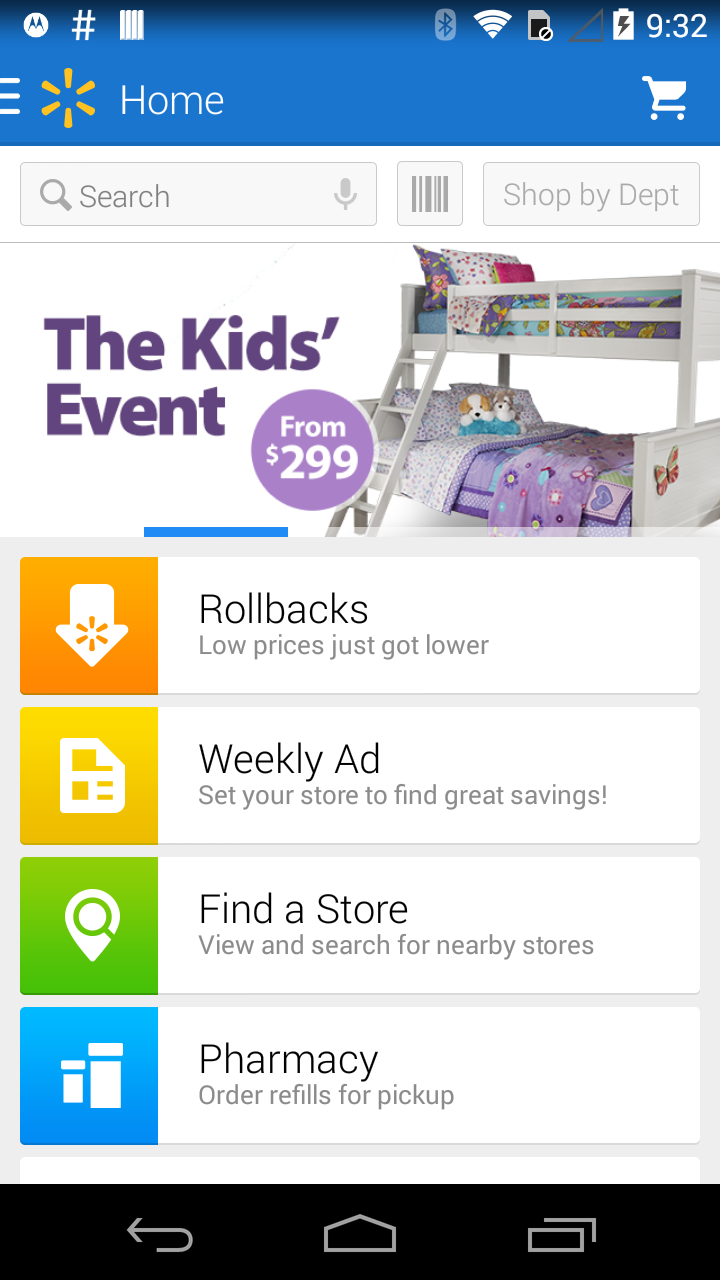
\includegraphics[width=0.3\columnwidth]{img/screen1.png}
    }
    \subfigure[Screen 2.]{
    \label{fig:screen2}
    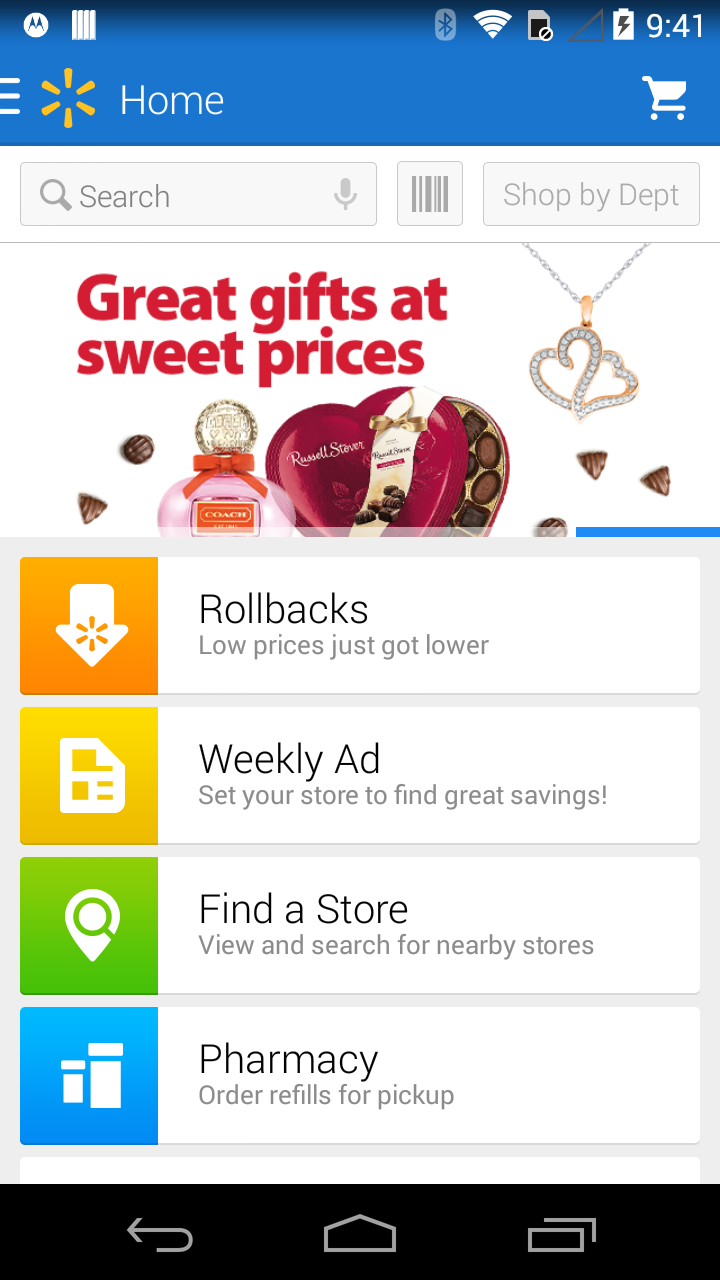
\includegraphics[width=0.3\columnwidth]{img/screen2.png}
    }
    \subfigure[Difference for Screens 1 and 2.]{
    \label{fig:diff12}
    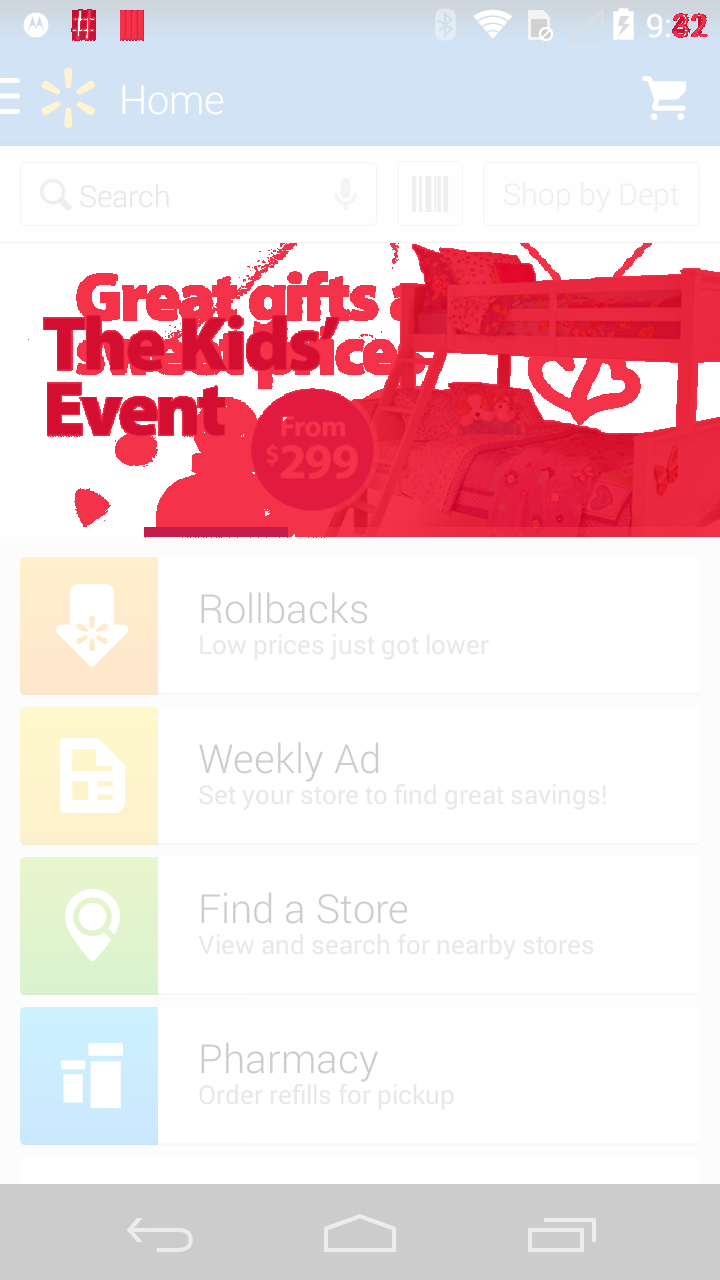
\includegraphics[width=0.3\columnwidth]{img/diff12.png}
    }

    \subfigure[Screen 3.]{
    \label{fig:screen3}
    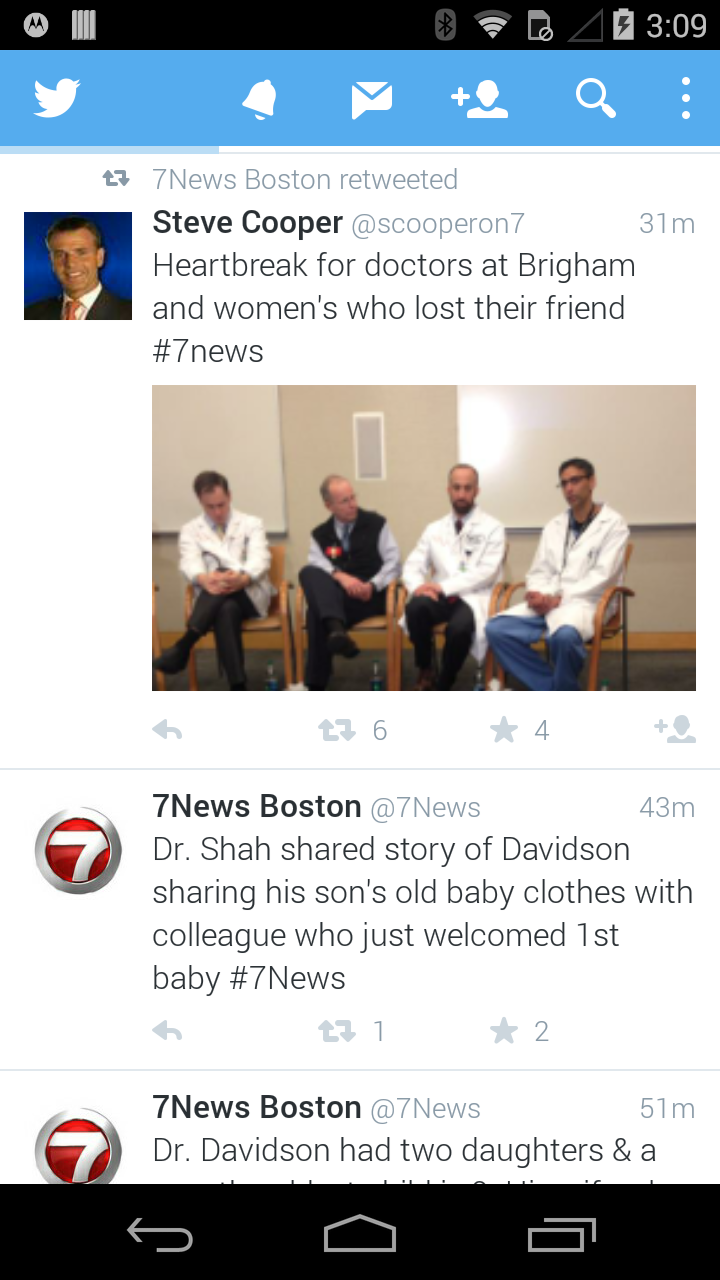
\includegraphics[width=0.3\columnwidth]{img/screen3.png}
    }
    \subfigure[Screen 4.]{
    \label{fig:screen4}
    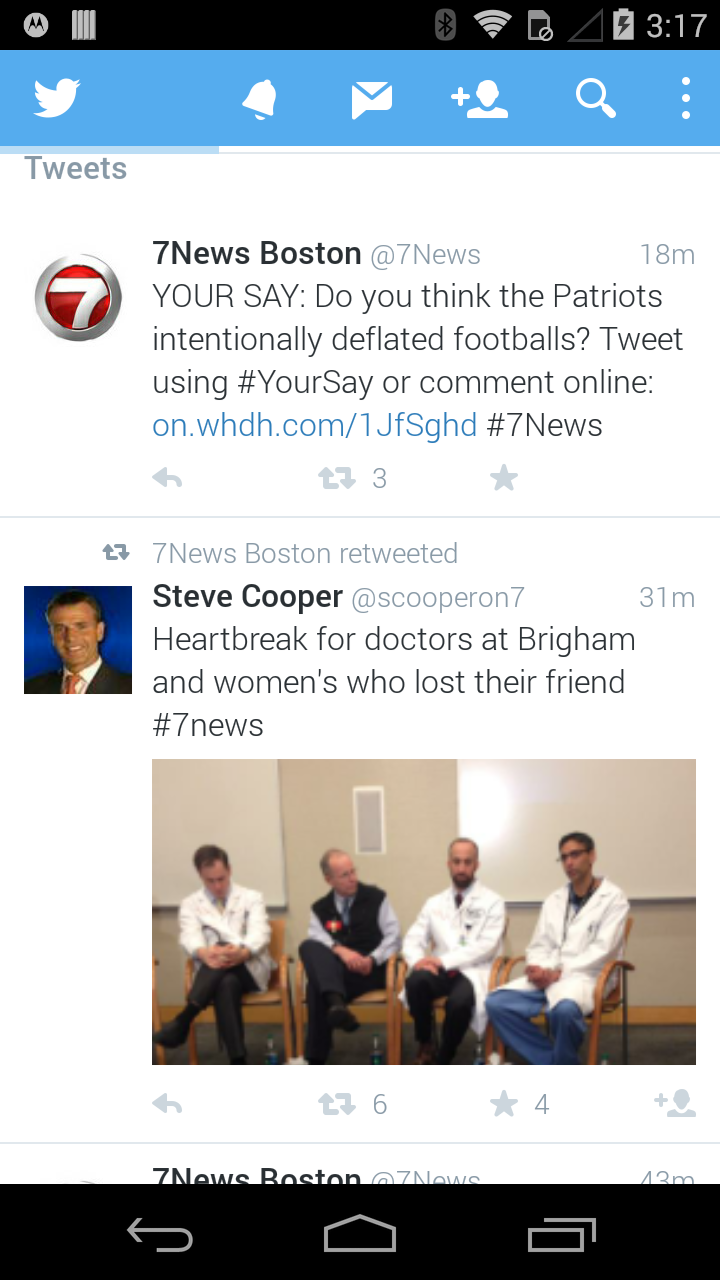
\includegraphics[width=0.3\columnwidth]{img/screen4.png}
    }
    \subfigure[Difference for Screens 3 and 4.]{
    \label{fig:diff34}
    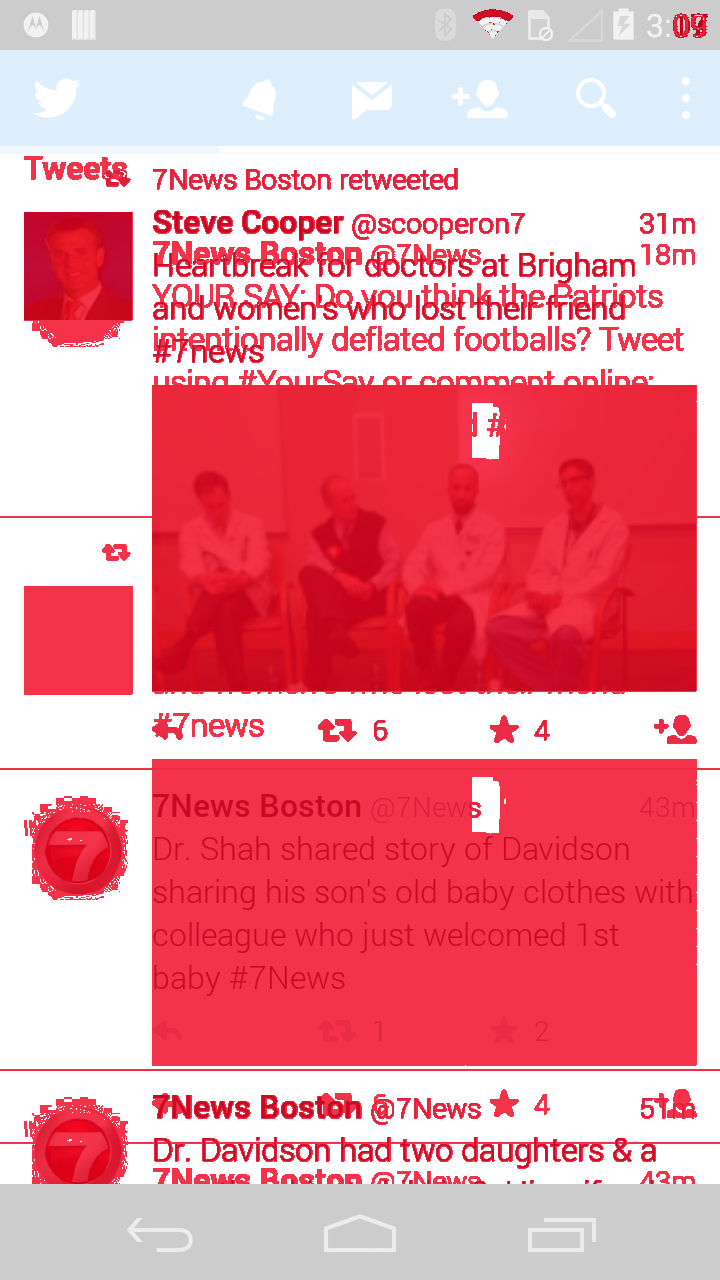
\includegraphics[width=0.3\columnwidth]{img/diff34.png}
    }
    \caption{Visual differences.}
    \label{fig:screenshots}
\end{figure}

For the comparison of application executions, we started by following the approach in~\cite{Hornyack:Han:Jung:Schechter:Wetherall:CCS11}, where screenshots from two different runs are placed side-by-side, 
along with a visual diff of each two corresponding images, as shown in Figure~\ref{fig:screenshots}, for 
the Walmart and twitter applications. 
We used the ImageMagick compare tool~\cite{imagemagick}
to produce the visual diff images automatically. 
We then manually scanned the produced output while ignoring differences in content of advertisement messages and the status of the device, deeming screenshots in Figures~\ref{fig:screenshots}(a) and (b) similar. 
We also ignored the exact content of widgets that are populated by applications in a dynamic manner and are designed to 
provide continuously updated information that is expected to differ between applications runs, such as tweets in Figures~\ref{fig:screenshots}(d) and (e). These two figures are thus also deemed similar.

In one out of ten analyzed cases, we had to revert to manual execution and comparison of the application runs.
That case involved interactions with a visual game that required rapid response time, 
thus the automated application execution was unable to provide reliable results. 


\vspace{0.1in}
\noindent 
{\bf Execution Methodology.}
We performed our study in three phases. In the first phase, we installed the original version of each analyzed 
application on a Nexus 4 mobile device running Android version 4.4.4.
We manually exercised the application, exploring all its functionality visible to us, and recorded the execution script that captured all triggered actions, as described above. 
We then re-installed the application to recreate a ``clean'' initial state and ran the produced execution script.  
We used screenshots collected during this run as the baseline for further comparisons. 

In the second phase, we used the Monitoring Transformation to produce a version of the original application that logs information about all existing and triggered connection statements. We ran the produced version using the execution script and collected the statistics about its communication patterns.  

In the third phase, we iterated over all \emph{triggered} connection statements, disabling them one by one, in order to assess
the necessity of each connection for preserving the user-observable behavior of the application. 
That is, we arranged all triggered connection statements in a list, in a lexical order and then applied the Blocking Transformation to disable the first connection statement in the list.   
We ran the produced version of the application using the recorded execution script and compared the obtained screenshots to the baseline application execution. If disabling the connection statement did not affect the behavior of the application, we marked it as \emph{non-essential}, kept it disabled for the subsequent iterations and proceed to the next connection in the list.
Otherwise, we marked the exercised connection as \emph{essential} and kept it enabled in the subsequent iterations.
We continued with this process until all connections in the list were explored.

%In all iterations, we also disabled all connections that were classified as non-triggered during the second phase. 
%That was done to improve the accuracy 
%of our analysis by proactively preventing applications from taking a new, previously unexplored, path when they detect connection failures. 
As the final quality measure, we manually introspected the execution of the version in which all non-essential connections
were blocked, to detect any  possible issues missed by the automated analysis.



\vspace{0.1in}
\noindent 
{\bf Subjects.} 
As the subjects of our study, we downloaded 15 top-popular applications available on the Google Play store in November 2014. 
We excluded from this list three chat applications, as our evaluation methodology does not allow assessing the usability of a chat application without a predictably available chat partner. 
We also excluded two applications whose asm-based instrumentation failed, most probably become they use language constructs that are not supported by that framework.

The remaining ten applications are listed in the first column of Table~\ref{tbl:applications}; their corresponding sizes are given in the second column of the table. 
We did not extend our dynamic analysis beyond these ten applications because the inspection of our findings indicated that we reached saturation: while it is clearly infeasible to explore all possible scenarios, we observed similar trends in all analyzed applications. As such, inclusion of additional ones was not expected to provide substantially new insights. 

\subsection{Results}
The quantitative results of the study are presented in columns~3--7 of Table~\ref{tbl:applications}. 
Column 3 and 4 of the table show that only a small number of connection statements encoded in the applications are, in fact, triggered dynamically. 
While some of the non-triggered statements can correspond to execution paths that were not explored during our dynamic application traversal, the vast majority of the statements originate in  
third-party libraries included in the application but only partially used, e.g., various Google services for mobile developers, advertising and analytics libraries and more.
In fact, we identified nine different advertising and analytics libraries used by the ten applications that we analyzed, 
and many times a single applications uses multiple such libraries.

An interesting case is the facebook application (row 3 in Table~\ref{tbl:applications}), where most of the application code is dynamically loaded at runtime from resources shipped within the apk file. 
Our analysis was unable to traverse this dynamically loaded code, and we thus excluded the application from the further analysis, noting that the only three connection statements that existed in the application jar file are never triggered. 

\begin{table}[t]
\caption{Communication Types.}
\label{tbl:statementTypes}
\centering
%\tabcolsep=1.5pt
\resizebox{\columnwidth}{!}{%
\begin{tabular}{|m{3.4cm}|C{2.3cm}|C{1.5cm}|}
\hline
%--------------------------------------------------------------------
                                                &  HTTP and Socket   & RPC \\
\hline
%--------------------------------------------------------------------
    Triggered                                   &  35 (30.7\%)       & 79 (69.3\%) \\
\hline
%--------------------------------------------------------------------
 Non-essential (total)                          &  18 (25.5\%)       & 53 (74.6\%) \\
\hline
%--------------------------------------------------------------------
 Non-essential (Google and Known A\&A Services) & 8 (17.7\%)         & 37 (82.2\%) \\
\hline
%--------------------------------------------------------------------
\end{tabular}
}% resizebox
\end{table}


\vspace{0.1in}
\noindent 
{\bf Classification of the Triggered Statements.}
Column 5 of Table~\ref{tbl:applications} shows the number of connection statements that we determined as non-essential during our study. 
Averaged for all applications, 65\% of the connections fall in that category. 
This means that only 35\% of the connection statements triggered by an application affect its observable behavior, 
when executed for the exact same scenario with the connection being either enabled or disabled (see column 6 of Table~\ref{tbl:applications}). 

Four of the analyzed applications contained advertisement material. For these applications, 71\% of the connections deemed  essential were used for advertising purposes, as shown in the last column of Table~\ref{tbl:applications}.

\conclusion{To answer RQ1, we conclude that non-essential communication often occur in real-world applications: 
65\% of the triggered connection statements can be deemed non-essential.}


Table~\ref{tbl:statementTypes} shows the distribution of the triggered connection statements 
into external communication performed via HTTP and sockets, and internal RPC communication. 
Overall, 30\% of all triggered connection statements correspond to external communication while 70\% -- to
internal ones, as shown in the second row of the table.
The breakdown is similar for the connection statements that we deemed non-essential: slightly more than 25\%
correspond to external communication and the remainder -- to the internal communication with services installed on the same device, as shown in the third row of Table~\ref{tbl:statementTypes}.

The last row of the table present statistic considering the communication with known advertisement and analytic services. The table shows that almost 18\% of the non-essential connections used for these purpose flow to the external services and 82\% -- to internal ones, which further communicate with external services to deliver the required content. 
Google services are commonly, but not exclusively, used by numerous applications. 

%\vspace{0.1in}
%\noindent 
%{\bf Information Leakages.}

\vspace{0.1in}
\noindent 
{\bf Lessons Learned.}
The collected statistics show that no principle distinction between essential and non-essential connections  
can be made just by considering connection types and their destinations. 
That observation is consistent with findings in~\cite{Hornyack:Han:Jung:Schechter:Wetherall:CCS11}, where authors 
show that blocking all messages to advertising and analytics services made more than 60\% of the applications either less functional or completely dysfunctional. 
We conclude that a more sophisticated 
technique for identifying the non-essential communication performed by the applications is required. 

We manually investigated binaries of several analyzed applications, to gain more insights into the way applications treat non-necessary connections of each of the identified type and communication target. 
We noticed that, in a large number of cases, connection failures are silently ignored by the applications without producing any visual indication to the user. 
That is, the exception triggered by the connection failure of a non-essential connection is either caught and ignored locally in the method that issues the connection or, more commonly, propagated upwards in the call stack and then ignored by one of the calling methods. 

In several cases, an error or warning message is written to the Android log file. However, this file is mostly used by  application developers and is rarely accessed by the end-user.

\conclusion{To answer RQ2, we conjecture that non-essential connections can be detected by inspecting connection failure paths. The lack of updates to GUI elements on the failure path is indicative for a connection being silently ignored by the application, thus being non-essential for the application execution.}











\section{Failure-Handling Analysis}
\label{sec:analysis}

\lstMakeShortInline[basicstyle=\scriptsize\ttfamily,keywordstyle=\color{DarkPurple},breaklines=false]+

In this section we describe the static analysis algorithm we employ to
automatically classify connections.  Given an Android application, the
static analysis classifies each statement that may invoke a
connection call as either {\it essential} or {\it non-essential}.
Intuitively, we define an essential connection statement, $s$, as
meeting either of the following criteria:
\vspace{-0.05in}
\begin{enumerate}[leftmargin=0.5cm]\setlength{\itemsep}{-0.05in}
\item{\bf User-Interface Cue}: When $s$ triggers an error, the user
may be notified of the error via a user interface cue during error
handling.
\item {\bf Program Exit}: When $s$ triggers an error, the program 
   may stop executing.  
\end{enumerate}
\vspace{-0.05in}
\noindent Conversely, a non-essential connection call does not meet
either of the two criteria.  

Android applications are developed in Java, and program execution
follows the semantics of Java. In an Android application, each
connection call $s$ may generate an exception (of dynamic type $e$)
that reaches a subset of the program's \lstinline!catch! blocks.  At
runtime, when $e$ is triggered by $s$, the executing method's trap
table is consulted, and if no \lstinline!catch! blocks are defined to
handle $e$ at $s$, then $e$ is passed back up the stack to the
calling method at the calling statement, and the process repeats.  If
the Android runtime is returned to during the stack unwinding, the
application is typically exited with an error.  


\begin{figure}
\begin{lstlisting}[numbers=left, escapeinside={(*@}{@*)},basicstyle=\ttfamily\scriptsize]
public class ApplicationClass {
    void f() {
        try {
            g();
            (*@{\it stmtA};@*)
        } catch (AdvertisingException e) {
            (*@{\it stmtB};@*)
        }
        (*@{\it stmtC};@*)
    }
}
public class AdvertisingAPIClass {
    void g() throws AdvertisingException {
        try {
            (*@{\it stmtD};@*)
            connect();  //throws RemoteException (*@\label{connect-fig-line}@*)
            (*@{\it stmtE};@*)
        } catch (RemoteException e) {
            (*@{\it stmtF};@*)
            throw new AdvertisingException();            
        }        
        (*@{\it stmtG};@*)
    }
}
\end{lstlisting}
\vspace{-0.2in}
\caption{\label{fig:failure-handling}An example of failure handling.
% of
%  of a connection call at line ~\ref{connect-fig-line}.  Statements
%  {\it stmtF}, \lstinline!throw new! \lstinline!AdvertisingException()!, and {\it stmtB}
%  are in the failure handling of this statement for exception \lstinline!RemoteException!.
}
\vspace{-0.1in}
\end{figure}

\begin{description}[leftmargin=0cm,listparindent=0pt,itemindent=0cm]
\item \textsc{\bfseries{Definition (Rethrown Exception)}}.  A
rethrown exception occurs when a \lstinline!catch! block catches an
exception, but before the block is exited, a statement reachable from
the block explicitly throws the same exception object, or throws a new
exception object.  The process of searching the stack for a handler
begins anew.

\item \textsc{\bfseries{Definition (Failure Handling)}}. The failure
  handling of a connection call $s$ for exception type $e$ is defined
  as the execution path that starts when an exception of type $e$
  propagates to connection call $s$ and ends when the {\it last}
  \lstinline!catch! block is exited that handles $e$ or a rethrown
  exceptions of $e$.
\end{description}

Intuitively, the failure handling of $s$ on $e$ is the computation
that handles $e$ and any failure triggered by the handling of $e$
(through rethrown exceptions).  Failure handling is finished when all
exceptions triggered by $e$ are handled and flow returns to normal
execution.  

Figure~\ref{fig:failure-handling} give a simplified representation of
failure handling pattern that we observed in the twitter application.
Method \lstinline!f! invokes method \lstinline!g!.  In \lstinline!g!,
a connection call is encountered on line~\ref{connect-fig-line};
assume during execution this connection call throws a
+RemoteException+.  The failure handling for this
connection call and exception is the set of statements:
{\it stmtF}, \lstinline!throw new! +AdvertisingException()+,
and {\it stmtB}.  These statements are executed from the start of the
handling of thrown \lstinline!RemoteException! to the end of the
handling of the rethrown \lstinline!AdvertisingException!.

\begin{description}[leftmargin=0cm,listparindent=0pt,itemindent=0cm]
\item \textsc{\bfseries{Problem}}: Analyze each connection call,
$s$, in an Android application to determine whether the application
could possibly exit on a failure at $s$ or could modify the user
interface during a failure handling path of $s$.
\end{description}

To solve this problem statically, our failure-handling analysis
conservatively calculates all possible failure handling for exceptions
that denotes connection failure for each connection call in the
application.  If there exists a failure-handling path of $s$ on $e$
that may include a call to a method that notifies the user of the
failure, then $s$ is considered essential.  If it is possible for $e$,
when triggered at $s$, to propagate back up the stack to the Android
runtime, $s$ is considered essential.

\subsection{Static Analysis of Android Applications}

%% Android applications are developed in Java and compiled to Dalvik
%% executable format (dex) byte code.  Android applications are
%% distributed as packages that do not include the Java source; packages
%% include only the dex byte code and application resources such as
%% images, sounds, and GUI declarations.  
Static analysis of Android
applications is notoriously difficult because of issues
including~\cite{Gordon:Kim:Perkins:Gilham:Nguyen:Rinard:NDSS15}:

\begin{itemize}[leftmargin=0.5cm]\setlength{\itemsep}{-0.05in}

\item Android applications execute in the context of the Android API
  and runtime.  The application thus represents an incomplete program.
  
\item The Android API and runtime comprises multiple millions of lines of
  code implemented in multiple programming languages.  Furthermore,
  much of the implementation is left for device manufactures to
  implement, and is thus proprietary and closed-source. 

\item Applications are event-driven and dynamic by nature.
  Applications define event handlers for possible runtime events that
  are triggered in the Android runtime, and passed to the application
  for handling. 

\item Applications interact heavily with the Android API.  The Android
  API includes most of the Java standard library, plus additional
  utility and resource access classes.

\item Android application packages typically ship with third-party
  libraries for performing operations such as advertising, analytics,
  and interaction with remote services.  These libraries are commonly
  large, obfuscated, and include heavy use of reflection.

\end{itemize}

It is not feasible for a static analysis to include analysis of the
source code of the Android runtime and API because of the size and
multi-language nature of this code base.  Thus static analysis must
either model the Android application execution environment, or account
for possible dynamic program behaviors with conservative analysis
choices; otherwise some runtime behaviors could be unconsidered.
Precise, whole-program analysis runs the high-risk of missing dynamic
program behavior and not scaling to real-world Android
application~\cite{Gordon:Kim:Perkins:Gilham:Nguyen:Rinard:NDSS15}.

Our analysis employs a class hierarchy analysis (CHA)~\cite{Dean1995}
to build a call graph with refinement achieved by intra-procedural
data-flow analysis.  After much experimentation with higher precision,
though brittle, points-to analysis techniques, this analysis
combination gave us the best performance for the classification task.
We augment the call graph to account for reflected method calls, and
conservatively account for exceptions that can be thrown by native
code.  Our failure-handling analysis over-approximates the runtime
behaviors of the applications, and under-approximates the connection
calls that could be non-essential.

The presented analysis has the following limitations. Dynamically
loaded code is not be considered.  The analysis considers only checked
exceptions.  A best-effort, though aggressive, policy is used to
account for reflection semantics; this policy could miss possible
runtime semantics.

Our analysis is implemented in the Soot Java Analysis
Framework~\cite{Vallee-Rai2000} and utilizes libraries and the Android
API model provided by
DroidSafe~\cite{Gordon:Kim:Perkins:Gilham:Nguyen:Rinard:NDSS15}. The
presentation of the analysis below assumes the application is
represented in the Jimple intermediate language~\cite{Vallee-Rai2000}.

\vspace{-0.05in}
\subsection{Call Graph Construction}

%%  A call graph represents the possible dynamic calling
%% relationship between methods of the application.  Each node represents
%% a method, and each edge, $(f,g)$ indicates that $f$ may call $g$ at
%% run time.

Our algorithm first computes a static call graph based on CHA
analysis. To compute a call graph, we augment the application code with the
DroidSafe Android Device Implementation
(ADI)~\cite{Gordon:Kim:Perkins:Gilham:Nguyen:Rinard:NDSS15}.  The ADI
is a Java-based model of the Android runtime and API that attempts to
present full runtime semantics for commonly-used classes of the
runtime and API.  Our call graph construction does not traverse into
Android API methods.  However, we found it necessary to account for
API calls that immediately jump back into the application.  For
example, if an application method, $m$ calls
\lstinline!Thread.start()! on a receiver that is an application class,
$t$, we found it necessary to add the edge to the call graph ($m$,
$t$.\lstinline!run()!).  This includes the started thread $t$ in
failure handler if $m$ is encountered.

To achieve this in general, we add to the call graph edges of the type
($m$, $n$) where there is an edge ($m$, \lstinline!api-method!), the
call of \lstinline!api-method! is passed a value that is a reference
to an application class, and \lstinline!api-method! calls method $n$
on the passed application class value.  This strategy adds to our
callgraph the edges for the \lstinline!Thread.start()! to the
\lstinline!Thread.run()! discussed above.

Furthermore, the call graph is augmented to account for reflected
method calls in the application using the following policy.  When a
reflected call is found, we add edges to the graph that target all
methods of the same package domain as the caller (e.g.,
\lstinline!com.google!, \lstinline!com.facebook!).  The edges are pruned by the
following strategy: if the number of arguments and argument types to
the call can be determined using a def-use analysis~\cite{Aho2006},
then we limit the edges to only targets that have the same number and
types of arguments.  This strategy works well for us in
practice and aggressively accounts for reflection semantics.

%\vspace{-0.05in}
\subsection{Failure Handler Analysis}
We organize the static failure-handling analysis as a recursive
traversal on the call graph for ease of understanding.  An iterator
over all application statements calls the analysis separately for the
combination of each statement in the application that could target a
connection call and an exception that indicates communication failure.
Table~\ref{tbl:connections} lists the target methods that we consider
connection calls and each method's associated failure exception.

%resize line numbers
\algrenewcommand\alglinenumber[1]{\scriptsize #1:}
\begin{figure}
\scriptsize
\begin{algorithmic}[1]
\algblockdefx[HEADER]{inputdef}{outputdef}[1]%
{\textbf{Input}: #1}[1]{\textbf{Output}: #1}
\Procedure{FindCatches}{meth, stmt, ex, visiting, stack, cg}

\If {(stmt, ex) $\in$ visiting || (stmt, ex) $\in$ essential}
    \State \textbf{return}
\EndIf

\State visiting $\gets$ visiting $\cup$ (stmt, ex)

\State catchBlockStart $\gets$ \textsc{FindCompatCatch}(meth, stmt, ex)

\If {catchBlockStart $=$ \textbf{null} }
\label{alg:no-local-hander-start}
\If {\textsc{IsEventHandler}(meth)}
\label{alg:event-handler-line}
\State essential $\gets$ essential $\cup$ (stmt, ex)
\State \textbf{return}
\EndIf

\For { (predStmt, predMeth) $\in$ \textsc{GetPreds}(cg, meth)}
\If {stack $\neq \emptyset$ \textbf{and} (predStmt, predMeth) $\neq$
  \textsc{Peek}(stack)} 
\label{alg:stack-test-line}
\State \textbf{continue}
\EndIf 

\State newStack $\gets$ stack
\State \textsc{Pop}(newStack)
\label{alg:stack-pop-line}
\State \textsc{FindCatches}(predMeth, predStmt, ex, 
\State         \hspace{2cm}visiting, newStack, cg)

\If {(predStmt, ex) $\in$ essential}
\State essential $\gets$ essential $\cup$ (stmt, ex)
\State \textbf{return}
\EndIf
\label{alg:no-local-hander-end}
\EndFor

\Else 
\State catchStmts $\gets$ \textsc{GetCatchStmts}(catchBlockStart, meth)
\label{findcatches-analyze-call}
\State \textsc{AnalyzeHandling}(meth, stmt, catchStmts,
\State \hspace{2cm}visiting, $\emptyset$, stack, cg)
\EndIf

\EndProcedure
\end{algorithmic}
\vspace{-0.05in}
\caption{Find \lstinline!catch! blocks for exception thrown at statement.}\label{alg:findcatches}
\vspace{-0.2in}
\end{figure}

The analysis starts with the \textsc{FindCatches} procedure listed in
Figure~\ref{alg:findcatches}.  For each start of the analysis on a
statement and exception pair, $s$ and $e$, respectively, the procedure
first consults $s$'s containing method to find an appropriate
\lstinline!catch!; if $e$ is not caught locally, the analysis
recursively visits all direct predecessors of the method to find
\lstinline!catch! blocks that trap the call statement edge (lines
\ref{alg:no-local-hander-start}-\ref{alg:no-local-hander-end}).  For
  each predecessor, $p$, if a catch is not found that wraps the call
  edge, then $p$'s direct predecessors are visited, and so on.

\begin{figure}[t]
\begin{algorithmic}[1]
\scriptsize
\algblockdefx[HEADER]{inputdef}{outputdef}[1]%
{\textbf{Input}: #1}[1]{\textbf{Output}: #1}
\Procedure{AnalyzeHandler}{meth, exceptStmt, stmts, 
  visiting, handledStmts, stack, cg}
\If {stmts $\in$ handledStmts}
\State \textbf{return}
\EndIf
\State handledStmts $\gets$ handledStmts $\cup$ stmts

\For {each stmt $\in$ stmts}
\If {\textsc{HasInvoke}(stmt)}
\For {(succStmt, succMeth) $\in$ \textsc{GetSuccs}(cg, stmt)}

\If {\textsc{IsUIMethod}(succMeth)}
\label{alg:ui-method-found}
\State essential $\gets$ essential $\cup$ exceptStmt
\State \textbf{return}

\ElsIf {\textsc{IsNativeMethod}(succMeth)}
\label{alg:native-method-line}
\For {nativeEx $\in$ \textsc{GetThrowsExceptions}(succMethd)}
\State \textsc{FindCatches}(meth, stmt, nativeEx, visiting, stack, cg)
\EndFor

\Else
\label{alg:ah-app-method-call-start}
\State newStack $\gets$ stack
\State \textsc{Push}(newStack, (succStmt, succMeth))
\label{alg-push-stack-lines}
\State succStmts $\gets$ \textsc{GetBodyStmts}(succMeth)
\State \textsc{AnalyzeHandler}(succMeth, exceptStmt, succStmts,
\State \hspace{2cm}visiting, handledStmts, newStack, cg)
\label{alg:ah-app-method-call-end}
\EndIf 

\EndFor

\ElsIf {\textsc{IsThrowStmt}(stmt)}

\State rethrownTypes = $\emptyset$
\label{alg:found-throws-start}
\For {defStmt $\in$ \textsc{GetLocalDefs}(\textsc{GetOp}(stmt))}

\If {\textsc{IsAlloc}(defStmt)}
\State rethrownTypes $\gets$ rethrownTypes $\cup$ 
\State \hspace{2.5cm} \textsc{GetAllocType}(defStmt)
\ElsIf {\textsc{IsCaughtExceptionStmt}(defStmt)}
\State rethrownTypes $\gets$ rethrownTypes $\cup$ 
\State \hspace{0.5cm} \textsc{GetPossibleThrownTypes}(meth, defStmt)
\label{alg:getpossiblethrowntypes}
\Else
\label{alg:unknown-last-def-throw}
\State essential $\gets$ essential $\cup$ exceptStmt
\State \textbf{return}
\EndIf

\EndFor \label{alg:calc-rethrow-types-end}

\For {rethrownType $\in$ rethrownTypes}
\label{alg:findcatches-rethrown-line}
\State \textsc{FindCatches}(meth, stmt, rethrownType, visiting, stack,
cg)

\If {stmt $\in$ essential}
\label{alg:progagate-line}
\State essential $\gets$ essential $\cup$ exceptStmt
\State \textbf{return}
\EndIf
\EndFor
\label{alg:found-throws-end}
\EndIf

\EndFor

\EndProcedure
\end{algorithmic}
\caption{Analyze reachable statements during handling for UI
  interaction or rethrown exceptions.}\label{alg:analyzehandler}
\vspace{-0.05in}
\end{figure}

For each \lstinline!catch! that is found during the
\textsc{FindCatch}, handler analysis of the reachable statements of
the \lstinline!catch! block is performed (\textsc{FindCatch}, line
\ref{findcatches-analyze-call}).  Figure~\ref{alg:analyzehandler}
gives the listing of the handler analysis procedure
\textsc{AnalzyeHandler}. The analysis considers the reachable
statements inter-procedurally and flow-insens\-itively.  Handler
analysis searches for: (1) calls to application methods, (2)
\lstinline!throw! statements (3) calls to native methods, and (4)
possible calls to UI methods. When the analysis finds a call to an
application method, it pushes the current statement and method onto
the stack and recursive calls itself for the new method to analyze the
new method's statements (lines
\ref{alg:ah-app-method-call-start}-\ref{alg:ah-app-method-call-end}).
If analysis finds a \lstinline!throw!  statement, the handler analysis
spawns a new \textsc{FindCatches} analysis to find all the
possible handlers of each rethrown exception (lines
\ref{alg:found-throws-start}-\ref{alg:found-throws-end}).  If analysis
finds a call to a native method, we assume that it will throw all
exceptions it is defined to throw, handler analysis spawns a
\textsc{FindCatches} instance for each exception declared throws
(line~\ref{alg:native-method-line}).  If a call is encountered that
could target a UI method, then the statement that began the handler
analysis is considered essential since the error handling affects the
user interface (line~\ref{alg:ui-method-found}).

\textsc{FindCatches} and \textsc{AnalyzeHandler} maintain a set of
statement and exception pairs, essential, that records pairs that are
calculated as essential.  After all connection call statement and
exception pairs are analyzed, pairs not in the essential set are
considered non-essential.

\lstDeleteShortInline+

\lstMakeShortInline[basicstyle=\scriptsize\ttfamily,keywordstyle=\color{DarkPurple},breaklines=true]+



\lstDeleteShortInline+



The set of target methods that are considered as affecting the user
interface are listed in Table~\ref{tbl:ui}.  We also define all
overriding methods of the methods listed in the table as UI methods.

A stack of pairs of method call statement and method is maintained
during the analysis.  The analysis uses the stack to focus the handler
search in \textsc{FindCatches} after a method call has been performed
by a handler further up the stack. When we initiate the analysis for
a connection call, the stack is empty and the analysis in
\textsc{FindCatches} has to search all possible stacks (predecessor of
the containing method) for handlers of the connection statement's
exception.  However, once a handler is found, and the handler calls a
sequence of methods that ends in a possible rethrown exception, the
sequence of methods defines the only stack that should be searched for
a handler of the rethrown exception.  The stack is pushed on line
\ref{alg-push-stack-lines} of \textsc{AnalyzeHandler} for each method
call of a reachable handler code.  During the handler search of the
execution stack in \textsc{FindCatches}, the
stack is consulted to guide the search on line
\ref{alg:stack-test-line}, only visiting the edge is at the head of
the stack. The stack is popped when visiting a caller method of the
current method in \textsc{FindCatches} line~\ref{alg:stack-pop-line}.

During handler search in \textsc{FindCatches}, if no handler is found
locally, and the method is a possible entry point called from the
Android runtime, then we conservatively calculate that the exception
and excepting statement could cause application exit, so the pair is
added to the essential set (line~\ref{alg:event-handler-line} of
\textsc{FindCatches}). 

During handler analysis, if a \lstinline!throw! statement is
encountered in reachable code of a handler, the analysis needs to
determine the possible type of the thrown value, and then start a new
search for the handler.  The \textsc{AnalyzeHandler} procedure
calculates local def-use chains for the method it is analyzing.  It
uses the local def-use information to calculate the types of the
exception.  In lines ~\ref{alg:found-throws-start} through
\ref{alg:calc-rethrow-types-end} the analysis considers all local
reaching definitions of the thrown value.  If an allocation statement
reaches, then add the allocated types to the possible types of
rethrown exceptions. If a caught exception statement\footnote{A caught
  exception statement is a statement that defines that start of a
  \lstinline!catch! block and assigns a local variable to the
  exception object caught by the block.}, $c$, reaches the
\lstinline!throw! statement, then the \lstinline!try! block associated
with \lstinline!catch! block of $c$ is analyzed for all checked
exceptions that could be thrown.  This is performed in
\textsc{GetPossibleThrownTypes} call on line
\ref{alg:getpossiblethrowntypes} of \textsc{AnalyzeHandler}.

If any other type of statement is a definition that reaches the thrown
value, then the analysis cannot determine the exception type and the
connection call (or rethrown exception statement) is considered
essential (line \ref{alg:unknown-last-def-throw}).  If only
allocations and caught exception statements reach the thrown value,
then the handler analysis spawns a new \textsc{FindCatches} instance
to analyze the failure handling.  The classification of the thrown
statement is propagated to the current excepting statement in
line \label{alg:progagate-line} of \textsc{AnalyzeHandler}.

\begin{figure}[t]
\begin{algorithmic}[1]
\scriptsize
\Procedure{GetPossibleThrownTypes}{meth,stmt}
\State thrownTypes = $[]$
\State tryStmts = \textsc{GetTryBlock}(meth,stmt)

\For {tryStmt $\in$ tryStmts}

\If {\textsc{IsThrowStmt}(tryStmt)}

\For {defStmt $\in$ \textsc{GetLocalDefs}(\textsc{GetOp}(stmt))}
\If {\textsc{IsAlloc}(defStmt)}
\State rethrownTypes $\gets$ rethrownTypes $\cup$ 
\State \hspace{1cm} \textsc{GetAllocType}(defStmt)
\ElsIf {\textsc{IsCaughtExceptionStmt}(defStmt)}
\State reThrownTypes $\gets$ rethrownTypes $\cup$
\State \hspace{1cm} \textsc{GetPossibleThrownTypes}(meth, defStmt)
\Else 
\State \textbf{return} $\emptyset$
\label{alg:getpossiblethrown-return-null}
\EndIf
\EndFor

\ElsIf {\textsc{HasInvoke}(tryStmt)}

\For {(succStmt, succMeth) $\in$ \textsc{GetSuccs}(cg, tryStmt)}
\State thrownTypes $\gets$ thrownTypes $\cup$ 
\State \hspace{1cm}\textsc{GetThrowsExceptions}(succMeth)
\EndFor

\EndIf

\EndFor

\State \textbf{return} thrownTypes

\EndProcedure
\end{algorithmic}
\caption{Calculate exception types caught at statement.\label{alg:GetPossibleThrownTypes}}
  \vspace{-0.1in}
\end{figure}

\begin{table}[t]
\small
\renewcommand*{\arraystretch}{1.3}
\caption{Considered UI Elements.}
\label{tbl:ui}
\centering
\tabcolsep=1.5pt
%\resizebox{\columnwidth}{!}{%
\begin{tabular}{|l|P{3.7cm}|P{4cm}|}
\hline
& \textbf{Class or Interface} & \textbf{Methods} \\
\hline
1. & +android.app.Dialog+                                 & +setContentView+ \\
2. & +android.support.v7.app.ActionBarActivityDelegate+  & +setContentView+ \\
3. & +android.view.View+                                  & +onLayout+, +layout+, +onDraw+, +onAttachedToWindow+ \\
4. & +android.view.ViewGroup+                             & +addView+, +addFocusables+, +addTouchables+, +addChildrenForAccessibility+ \\
5. & +android.view.ViewManager+                           & +addView+, +updateViewLayout+ \\
6. & +android.view.WindowManagerImpl.CompatModeWrapper+  & +addView+ \\
7. & +android.webkit.WebView+                             & +loadData+, +loadDataWithBaseURL+, +loadUrl+ \\
8. & +android.widget.TextView+       & +append+, +setText+ \\
9. & +android.widget.Toast+        & +makeText+ \\
\hline
\end{tabular}
%}%resizebox
\end{table}

Figure~\ref{alg:GetPossibleThrownTypes} gives the algorithm for
\textsc{GetPossibleThrownTypes}.  First, the method calculates the
\lstinline!try! block that associates with the \lstinline!catch! block
that encloses $stmt$. Next, the procedure examines \lstinline!throw!
and call statements of the \lstinline!try!.  For a call statement, the
procedure adds to the return list all exception types declared throws
by all methods that the call can target.  For a \lstinline!throw!
statement, the reaching definitions of the thrown value are
calculated.  If the reaching definition is an allocation, then add to
the return list the type of the allocation.  If the reaching
definition is a caught exception statement, then
\textsc{GetPossibleThrownExceptions} recursively calls itself to find
the nesting try block statements and continue the calculation.  If a
definition of any other statement type can reach the thrown value,
then the procedure returns null to denote that it cannot calculate the
thrown type (line~\ref{alg:getpossiblethrown-return-null}).  This
situation causes the examined connection call or rethrown statement in
\textsc{AnalyzeHandler} to be labeled essential (we have not included
the code in the algorithms to propagate this situation to the
essential set, though it is in our implementation).


\subsection{Helper Procedures}

The analysis employs the following helper procedures: 

\begin{description}[leftmargin=0cm,listparindent=0pt,itemindent=0cm]

\item \textsc{FindCompatCatch}($meth$,$stmt$,$ex$): Return the first
  statement of the \lstinline!catch! block that will handle an
  exception of type $ex$ thrown at statement stmt in method meth.

\item \textsc{IsEventHandler}($meth$): Return true if method $meth$
  overrides a method defined in the Android API.  This method
  over-approximates the methods that can be called by the Android
  runtime to handle events.

\item \textsc{GetCatchStmts}($stmt$,$meth$): Given the start of a
  \lstinline!catch! block defined in the trap table of method $meth$,
  return all statements that were defined in the source code for the
  \lstinline!catch! block of $stmt$.  Since the dex bytecode does not
  provide the ending statement of traps, we need to calculate the
  extent of the catch block.  \textsc{GetCatchStmts} takes advantage
  of the property that Java compilers do not produce code that jumps
  from outside of the catch block into the middle of a catch block.
  So to calculate the \lstinline!catch! block's extent,
  \textsc{GetCatchStmts} (1) produces a control flow graph (CFG) for
  $meth$, (2) colors all statements reachable from $stmt$ in the CFG,
  (3) for each statement, $c$ of $meth$, if all predecessors of $c$ in
  the CFG are colored then $c$ is included in the set of statements
  that are returned ($stmt$ is also included in the return set). This
  method calculates an over-estimation of \lstinline!catch! block
  extents, e.g., it includes \lstinline!finally! blocks.

\item \textsc{GetTryBlock}($meth$,$stmt$): Given a statement $stmt$
  that begins a \lstinline!catch! block in method $meth$, return the
  list of statement of try block associated with the enclosing
  \lstinline!catch! block of $stmt$.

\end{description}


\begin{table}[t]
\caption{Comparison with the Manually Established Results.}
\label{tbl:eval}
\centering
\tabcolsep=2.0pt
\resizebox{1.0\columnwidth}{!}{%
\begin{tabular}{|l|C{2.7cm}|C{2.7cm}|C{1.9cm}|}
\hline
\multirow{2}{*}{\textbf{Applications}} & \multicolumn{2}{c|}{\textbf{Correctly detected non-essential}} & \multirow{2}{1.4cm}{\textbf{Execution time}} \\
\cline{2-3}
                                & Precision         & Recall            &    \\
\hline
%--------------------------------------------------------------------
air.com.sgn.cookiejam.gp  & 1/1 (100.0\%)  & 1/2 (50.0\%)  & 1min 50s \\
com.crimsonpine.stayinline  & 2/2 (100.0\%)  & 2/2 (100.0\%)  & 1min 52s \\
com.devuni.flashlight   & 1/2 (50.0\%)  & 1/1 (100.0\%)  &          \\
com.emoji.Smart.Keyboard  & 2/2 (100.0\%)  & 2/2 (100.0\%)  &          \\
com.grillgames.guitarrockhero & 1/1 (100.0\%)  & 1/14 (7.1\%)  & 2min 54s \\
com.jb.emoji.gokeyboard   & 4/4 (100.0\%)  & 4/7 (57.1\%)  &          \\
com.pandora.android    & 4/4 (100.0\%)  & 4/9 (44.4\%)  & 2min 13s \\
com.spotify.music    & 1/1 (100.0\%)  & 1/3 (33.3\%)  & 2min 18s \\
com.twitter.android    & 1/1 (100.0\%)  & 1/3 (33.3\%)  & 2min 33s \\
com.walmart.android    & 3/3 (100.0\%)  & 3/5 (60.0\%)  & 2min 17s \\
net.zedge.android    & 3/4 (75.0\%)  & 3/4 (75.0\%)  & 2min 31s \\
\hline
%--------------------------------------------------------------------
Average       & 23/25 (93.2\%) & 23/52 (60.0\%) & 2min 18s \\
\hline
%--------------------------------------------------------------------
\end{tabular}
}% resizebox
\end{table}

\section{Experiments}
\label{sec:evaluation}
To establish the quality of our static analysis technique, we first evaluate its precision and recall on the ``truth set'' established during our in-depth case study (see Section~\ref{sec:study}). 
We then apply our analysis on 500 top-popular Android applications from Google Play. 
We select XX of these application for further investigation: we inject failures in all connection statements identified as non-essential by our static analysis, as described in Section~\ref{sec:study}, 
and they employ humans to check whether these are any observable differences between the original and the modified application, 
Finally, we use the 

For the remaining ones, we use the gathered information to report on common patterns of non-essential communication in the wild.

\subsection{Evaluation of the Static Analysis}
For our evaluation, we limit the set of results reported by the static analysis to those that were, in fact,
 triggered during our dynamic study (see Table~\ref{tbl:applications} in Section~\ref{sec:study}): these are the connection statements for which we have reliable information to compare against. 
We assess the results, for each application individually and averaged for all applications, using the metrics below. The results are summarized in Table~\ref{tbl:eval}.

\begin{enumerate}[leftmargin=0.5cm]%\setlength{\itemsep}{-0.05in}
\item
\emph{Expected}: the size of the predetermined expected result, i.e., the number of connections listed as non-essential in Table~\ref{tbl:applications}.
\item
\emph{Reported}: the number of connections deemed as non-essential by the static analysis. 
\item
 \emph{Correct}: the number of non-essential connections correctly identified by the static analysis, i.e., those that were deemed as non-essential in the dynamic study as well.
% reported by the technique.\\
\item
\emph{Precision}: the fraction of relevant results among those reported,
% by the technique,
 calculated as \emph{$\frac{\text{Correct}}{\text{Reported}}$}. 
\item
\emph{Recall}: the fraction of relevant results among those expected, calculated as
\emph{$\frac{\text{Correct}}{\text{Expected}}$}.
%\item
%\emph{F-measure}: a harmonized measure combining precision and recall, whose
%value is high if both precision and recall are high, calculated as \emph{$\frac{2 \times \text{Precision} \times \text{Recall}}{\text{Precision} + \text{Recall}}$}. This measure is usually used to evaluate the accuracy of a technique as
%it does not allow trading-off precision for recall and vise versa.
\item \emph{Execution time}: the execution time of the analysis, measured by averaging results of
three runs on an Intel\textsuperscript{\textregistered} Xeon\textsuperscript{\textregistered} CPU E5-2690 v2 @ 3.00GHz machine running Ubuntu 12.04.5. The machine was configured to use at most 16GB of heap and to perform no parallelization for a single application, i.e., each application uses one core only.
\end{enumerate}
  
As can be seen in the second and the third columns of Table~\ref{tbl:eval}, the overall averaged precision of our analysis is 83.3\%. 
The analysis correctly identified 64 non-essential connections out of the total 82 reported. 
18 connections were mis-classified, out of which 16 correspond to \emph{optional} application behaviors, i.e.,
when connection failures are indeed ignored and the applications proceed without the missing information. The 
remaining two cases correspond to a \emph{stateful} communication within the application. 
The details of each of these cases are given below: 

\begin{itemize}[leftmargin=0.5cm]%\setlength{\itemsep}{-0.05in}
\item 13 connections are used for presenting \emph{optional} advertisement content: 
3 in the \emph{net.zedge.android} application, and 
5 in \\
\emph{com.crimsonpine.stayinline} and \emph{com.grillgames.guitarrockhero} each.
\item 3 connections correspond to 
\emph{optional} application behaviors: 2 in the \emph{com.walmart.android} application, responsible for providing location-aware search, and 1 in the \emph{com.spotify.music} application, responsible for enhancing the presented album with images.
\item 2 connections, both in \emph{com.spotify.music}, correspond to \emph{stateful} communication within the application. 
Blocking each of these connections, individually, harms the application's search capabilities.
\end{itemize}

Considering the advertisement information as non-essential gives an overall average precision of 90.8\%, as shown in column 4 of Table~\ref{tbl:eval}. 
That is, depending on the user's perspective, 
between 83\% and 90\% of the cases identified as non-essential by the static analysis indeed do not affect the behavior of the applications. 

While designed to be conservative, our analysis is able to correctly identify 64 out of 106 connection statements deemed non-essential in the empirical study, resulting in the overall recall of 63.8\% (column 3 in Table~\ref{tbl:eval}). Considering advertisement non-essential results in a slight increase in recall, to 64.6\% (column 5 in Table~\ref{tbl:eval}).
The technique correctly identifies the majority of non-essential connections.

Finally, the last column of table Table~\ref{tbl:eval} shows that our analysis is highly efficient -- it runs in a matter of minutes even on large applications. 

\subsubsection{Usability assessment}

We recruted two users and paired each one up with one of the authors of this paper.  Each pair was given two devices - one running. 
The users simultaneously executed the same app on both devices and noted all differences.

Each app was executed for 5 to 10 mins. Sign in and in app purchases.

Subjects.

Results.

\conclusion{To answer RQ3, we conclude that a static analysis can be applied for an accurate detection of non-essential connections. Our highly scalable technique features up to 90\% precision and 64\% recall, respectively.}



%\begin{table}[t]
%\renewcommand*{\arraystretch}{1.3}
%\caption{Top 20 Non-Essential Communication Callers.}
%\label{tbl:callers}
%\centering
%\tabcolsep=1.5pt
%\resizebox{\columnwidth}{!}{%
%\begin{tabular}{|r|P{3.2cm}|P{3.5cm}|C{1.8cm}|C{1.8cm}|}
%\hline
%%--------------------------------------------------------------------
%  &                 & Description                       & Used in \# (\%) of Apps   & (\%) from Total Non-Essential Calls in a App (Avg.)  \\
%\hline
%%--------------------------------------------------------------------
% 1. & com.google.android.gms       &  Google mobile services        & 403 (80.6\%) & 91.0\% \\
% 2. & com.facebook          &  Facebook services         & 190 (38.0\%) &  2.4\% \\
% 3. & com.android.\newline{}vending.billing   &  Google in-app billing        & 139 (27.8\%) &  1.6\% \\
% 4. & com.chartboost.sdk        &  Gaming services          & 116 (23.2\%) &  0.8\% \\
% 5. & com.flurry.sdk         &  Advertising, monetization and analytics services & 79 (15.8\%) &  3.9\% \\
% 6. & com.millennialmedia.\newline{}android   &  Advertising, monetization and analytics services & 76 (15.2\%) &  1.9\% \\
% 7. & com.mopub.mobileads        &  Advertising, monetization and analytics services & 70 (14.0\%) &  1.1\% \\
% 8. & com.tapjoy          &  Advertising, monetization and analytics services & 47  (9.4\%) &  3.7\% \\
% 9. & com.bda.controller        &  PhoneGap game controller       & 23  (4.6\%) &  2.4\% \\
%10. & com.unity3d.\newline{}plugin.downloader   &  Gaming Services          & 21  (4.2\%) & 20.3\% \\
%%11. & com.outfit7.\newline{}talkingfriends.offers  &  Components of Outfit7 Android developers   & 16  (3.2\%) &  2.5\% \\
%%12. & com.google.android.\newline{}youtube.player  &  Google YouTube API         & 11  (2.2\%) & 16.5\% \\
%%13. & com.cleanmaster         &  Phone Booster and Antivirus app      & 8  (1.6\%) & 24.5\% \\
%%14. & com.ijinshan.kbackup        &  Cloud backup and restore app      & 3  (0.6\%) & 26.5\% \\
%%15. & cn.wps.moffice         &  Office app           & 1  (0.2\%) & 77.1\% \\
%\hline
%%--------------------------------------------------------------------
%\end{tabular}
%}% resizebox
%\end{table}

\begin{table}[t]
\renewcommand*{\arraystretch}{1.3}
\vspace{-0.15in}
\caption{Top 10 Non-Essential Communication Callers.}
\label{tbl:callers}
\centering
\tabcolsep=1.5pt
\resizebox{0.9\columnwidth}{!}{%
\begin{tabular}{|r|P{3.2cm}|P{3.5cm}|C{1.8cm}|C{1.8cm}|}
\hline
%--------------------------------------------------------------------
    &                         & Description                           & Used in \# (\%) of Apps  \\
\hline
%--------------------------------------------------------------------
 1. & com.google.android.gms            &  Google mobile services             & 403 (80.6\%)  \\
 2. & com.facebook                &  Facebook services               & 190 (38.0\%)  \\
 3. & com.android.\newline{}vending.billing     &  Google in-app billing             & 139 (27.8\%)  \\
 4. & com.chartboost.sdk             &  Gaming services                & 116 (23.2\%)  \\
 5. & com.flurry.sdk               &  Advertising, monetization and analytics services & 79 (15.8\%)  \\
 6. & com.millennialmedia.\newline{}android     &  Advertising, monetization and analytics services & 76 (15.2\%)  \\
 7. & com.mopub.mobileads             &  Advertising, monetization and analytics services & 70 (14.0\%)  \\
 8. & com.tapjoy                 &  Advertising, monetization and analytics services & 47  (9.4\%)  \\
 9. & com.bda.controller             &  PhoneGap game controller            & 23  (4.6\%)  \\
10. & com.unity3d.\newline{}plugin.downloader    &  Gaming Services                & 21  (4.2\%)  \\
%11. & com.outfit7.\newline{}talkingfriends.offers  &  Components of Outfit7 Android developers     & 16  (3.2\%)  \\
%12. & com.google.android.\newline{}youtube.player  &  Google YouTube API               & 11  (2.2\%)  \\
%13. & com.cleanmaster               &  Phone Booster and Antivirus app         & 8  (1.6\%)  \\
%14. & com.ijinshan.kbackup             &  Cloud backup and restore app          & 3  (0.6\%)  \\
%15. & cn.wps.moffice               &  Office app                  & 1  (0.2\%)  \\
\hline
%--------------------------------------------------------------------
\end{tabular}
}% resizebox
\end{table}

\subsection{Non-Essential Communication In the Wild}

We apply our technique on the 500 most popular Android application
downloaded from the Google Play store in January 2015.  Our goal is to
investigate how often non-essential communication occurs in real-life
applications and what are its most common destinations.

%\begin{table}[t]
%\caption{Analysis of the 500 Top-Popular Applications from Google Play.}
%\label{tbl:googlePlayApps}
%\centering
%\tabcolsep=1.5pt
%%\resizebox{\columnwidth}{!}{%
%\begin{tabular}{|l|C{2.8cm}|C{1.9cm}|}
%\hline
%%--------------------------------------------------------------------
%                    & Non-Essential     & Total          \\ % Exec. time
%\hline
%%--------------------------------------------------------------------
%Total (500 apps)    & 283,159 (84.2\%)  &  336,203       \\ % 23h 54min 1s
%Avg. per app        &   566.3           &  672.4         \\ %   2min 52s
%\hline
%%--------------------------------------------------------------------
%\end{tabular}
%%}% resizebox
%\end{table}

Our analysis reveals that 46.2\% of all connections encoded in these application can be considered non-essential (8,539 connection out of 18,480 in total).
These results are consistent with the observation of our empirical study described in Section~\ref{sec:study}.
%, showing that a large percent of connections
%made by applications can be considered non-essential.  In fact, even
%with our conservative analysis, 84\% of connections fall into that
%category.
%In Table~\ref{tbl:googlePlayApps}, we report on the number of
%non-essential connections found in these applications in total, and
%for an application on average.  These results confirm the observation
%of our empirical study, showing that a large percent of connections
%made by applications can be considered non-essential.  In fact, even
%with our conservative analysis, 84\% of connections fall into that
%category.
Table~\ref{tbl:callers} presents the top 10 packages in which
non-essential connections occur.  As the numbers are aggregated for
500 applications, it is not a surprise that Google Services, as well
as gaming, advertisement and analytics services, are on the top of the
list -- numerous applications use these services, as shown in the last
column of Table~\ref{tbl:callers}.  By manually investigating some of
the most-popular connections in reverse-engineered versions of the
applications, we observed that those connections are designed to be
``best-effort'' only. For example, an application might attempt to
obtain user-specific advertisement information, but continues with
generic advertisement if that attempt fails.  The prevalence of mobile
services and their ``best-effort'' behavior make us believe that it
would be beneficial if these services were designed to allow users to
select the level of support they wish to obtain, instead of relying
merely on connectivity for that purpose.

 
%The last column of the table shows the ratio of non-essential calls 
%made from a package out of the total number of non-essential calls, averaged for all applications that use the corresponding package, e.g., 403 in the case of Google Services. 
%Interestingly, the highest fraction of non-essential calls made by applications falls within this package. 
%There could be two reasons for this finding: first, applications commonly register for various Google services  services without eventually using
%them.


%Dead code comes from libraries. If 
%it is just not used by a specific application, but might be used by another one, so it is good to analaze it in any case


\conclusion{To answer RQ4, we conclude that non-essential communication is very common in real-life applications. 
Most such communication is performed with various mobile services that are designed to be ``best-effort only'', i.e., communication failures do not prevent 
successful application execution. Designing mobile services that allow the user to select the preferred level of support instead of relying merely on connectivity would be beneficial.}



\vspace{0.05in}
\section{Limitations and Threats to \\Validity}
\label{sec:limitations}
%In this section we discuss the limitations of our empirical study and our static technique for detecting non-essential connections.

%\vspace{0.05in}
%\noindent 
\subsubsection{Empirical Study}
Our empirical study has a dynamic nature and thus suffers from the well-known limitations of dynamic analysis: it does not provide an exhaustive exploration of an application's behavior.
%, thus the findings apply only to the execution paths explored during the analysis. 
Even though we made an effort to cover all application functionality visible to us, we might have missed some behaviors, e.g., those triggered under system settings different from ours. 
We attempted to mitigate this problem by performing all our dynamic experiments on the same device, at the same location and temporally close to each other.  
We also automated our execution scripts in order to compare behaviors of different variants under the same scenario and settings. 
We only report on the results comparing these similar runs.  

During our analysis, we disabled connections one by one, iterating over their list arranged in a lexicographic (i.e., semantically random) order. As such, we could miss cases when 
several connections can be excluded altogether, but not individually. 
Since exploring all connection state combinations is exponential, we opted for this linear approach that still guarantees correct, 
albeit possibly over-approximate results. Moreover, by focusing on individual connection statements, we cannot distinguish between multiple application behaviors
that communicate via the same statement in code. We thus conservatively deem a connection as essential if it is essential for at least one of such behaviors. 
%Exploring more sophisticated techniques for distinguishing between such different behaviors could be a subject of a possible future work.
 
Finally, our study only includes a limited number of subjects, so the results might not generalize to other applications.
We tried to mitigate this problem by not biasing our application selection but rather selecting top-popular applications from the Google Play store, and by ensuring that we observe similar communication patterns in all analyzed applications.

%\vspace{0.05in}
%\noindent 
\subsubsection{A Static Technique For Detecting Non-Essential Connections}
Our technique deems 
%\emph{optional} behaviors -- those when failing connections are ignored by the application, but successful connections result in presenting additional information to the user -- as non~essential. 
%As an application can proceed when optional behaviors are excluded, it is debatable whether they are really essential for the application functionality or not. 
%In fact, we believe that it is up to the users to decide whether an optional behavior is indeed essential for their needs. 
%%Towards this end, we plan to investigate approaches for differentiating between optional and ``truly non-essential'' behaviors as part of a future work. 
%
%Our technique also deems 
as non-essential \emph{stateful} communication that toggles
the state of a connection target but does not present any information to the user. 
In many cases, detecting such
communication statically is impossible because the code executed on
the target is unknown and unavailable. 
For a similar reason, in this work, we did not consider RPC communication with applications
installed on the same device. We might explore that direction as part of the future work. 
%When communication is
%performed via RPC within the same application, it is exceedingly
%costly for an analysis to determine, with precision, whether a
%connection (or set of connections) is stateful. 
%As such cases are
%rare, developing these approaches, orthogonal to our current analysis,
%is also left to future work.
 
Some of the non-essential connections that we identified statically might never be triggered dynamically. 
%In fact, our empirical study shows that only a small fraction of the connection statements in the analyzed applications were indeed triggered.
%Some of such connections belong to execution paths that were not explored during our dynamic application traversal.
A large percentage of these connections originate in  
third-party libraries that are included in the application but only partially used. 
As such, analyzing them is still beneficial as this code might be used in other applications.
%Nevertheless, our approach could be combined with techniques for detecting dead code, to prevent false-positive results. 

\section{Related Work}
\label{sec:related}
Work related to this paper falls into three main categories: (1)
user-centric analysis to identify spurious application behaviors (2)
information propagation in mobile applications, and (3) static
exception analysis for Java. 

\vspace{0.1in}
\noindent 
{\bf User-Centric Analysis for Identifying Spurious Behaviors in Mobile Applications.}
Huang et al.~\cite{Huang:Zhang:Tan:Wang:Liang:ICSE14} propose a technique, AsDroid, for identifying contradictions between a user interaction function and the behavior that it performs. 
This technique associates intents with certain sensitive APIs, such as HTTP access or SMS send operations, and tracks the propagation
of these intents through the application call graph, thus establishing correspondence between APIs and the UI elements they affect. 
It then uses the established correspondence to compare intents with the text related to the UI elements. Mismatches are treated as potentially stealthy behaviors. 
In our work, we do not assume that all operations are triggered by the UI
and do not rely on textual descriptions of UI elements.

CHABADA~\cite{Gorla:Tavecchia:Gross:Zeller:ICSE14} compares natural language descriptions of applications, clusters them by description topics, and then identifies outliers by observing API usage within each cluster. Essentially, this system identifies applications whose behavior would be unexpected given their description. Instead, our approach focuses on identifying unexpected behaviors given the actual user experience, not just the description of the application.

Elish et al.~\cite{Elish:Yao:Ryder:MOST12} propose an approach for identifying malware by tracking dependencies between the definition and the use of user-generated data. They deem sensitive function calls that are not triggered by a user gesture as malicious. However, in our experience, the absence of a data dependency between a user gesture and a sensitive call is not always indicative for suspicious behavior: applications such as twitter and Walmart can initiate HTTP calls to show the most up-to-date information to their user, without any explicit user request. Moreover, malicious behaviors can be performed as a side-effect of any user-triggered operation. We thus take an inverse approach, focusing on identifying operations that do not affect the user experience.

\vspace{0.1in}
\noindent 
{\bf Information Propagation in Mobile Applications.}
The most prominent technique for dynamic information propagation tracking in Android is TaintDroid~\cite{Enck:Gilbert:Chun:Cox:Jung:McDaniel:Sheth:OSDI10}, which detects flows of information from a selected set of sensitive sources to a set of sensitive sinks.
%TaintDroid is used, extended and customized by several follow-up research projects.
%For example, the Kynoid system~\cite{Schreckling:Posegga:Koestler:Schaff:WISTP12} extends it with user-defined security policies, which include temporal constraints on data processing as well as restrictions on
%destinations to which data is released.
Several static information flow analysis techniques for tracking propagation of information from sensitive sources to sinks have also been recently developed~\cite{
%Yang:Yang:WCSE12, Gibler:Crussell:Erickson:Chen:TRUST12, 
Arzt:Rasthofer:Fritz:Bodden:Bartel:Klein:Traon:Octeau:McDaniel:PLDI14,Gordon:Kim:Perkins:Gilham:Nguyen:Rinard:NDSS15,Klieber:Flynn:Bhosale:Jia:Bauer:SOAP14,Li:Bartel:Klein:Traon:Arzt:Rasthofer:Bodden:Octeau:McDaniel:CoRR14}.
The first two ensure accurate detection of information flows within a single application, while the last two -- across multiple applications. 

McCamant and Ernst~\cite{McCamant:Ernst:PLDI08} take a quantitative approach to information flow: they cast information-flow security to a network-flow-capacity problem and describe a dynamic technique for measuring the amount of secret data that leaks to public observers. 
Tripp and Rubin~\cite{Tripp:Rubin:SEC14} propose to extend the information flow analysis with a Bayesian notion of statistical classification, which conditions the judgment whether a release point is
legitimate on the evidence arising at that point, e.g., the similarity between the data
values about to be released and the data obtained via the source APIs. 

Our work is orthogonal and complimentary to all the above: while they focus on providing precise information flow tracking capabilities and detecting cases when sensitive information flows outside of the application and/or mobile device, 
our focus is on distinguishing between essential and non-essential flows. 

The authors of AppFence~\cite{Hornyack:Han:Jung:Schechter:Wetherall:CCS11} build up on TaintDroid and explore approaches for either obfuscating or completely blocking the identified cases of sensitive information release.
Their study shows that blocking all such cases renders more than 65\% of the application either less functional or completely dysfunctional, blocking cases when information flows to advertisement and analytics services ``hurts'' 10\% of the applications, and blocking the communication with the advertisement and analytics services altogether -- more than 60\% of the applications.
Our work has a complementary nature as we rather attempt to identify cases when communication can be disabled without affecting the application functionality. 
Our approach for assessing the user-observable effect of that operation is similar to the one they used though. 

Both MudFlow~\cite{Avdiienko:Kuznetsov:Gorla:Zeller:Arzt:Rasthofer:Bodden:ICSE15} and AppContext~\cite{Yang:Xiao:Andow:Li:Xie:Enck:ICSE15} build up on the FlowDroid static information flow analysis system~\cite{Arzt:Rasthofer:Fritz:Bodden:Bartel:Klein:Traon:Octeau:McDaniel:PLDI14} and propose approaches 
for detecting malicious applications by learning ``normal'' application behavior patterns and then identifying outliers. 
The first work considers flows of information between sensitive sources and sinks, while the second  -- contexts, i.e., the events and conditions, that cause the security-sensitive behaviors to occur. 
Our work has a complementary nature as we focus on identifying non-essential rather than malicious behaviors, aiming to preserve the overall user experience. 

Shen et al.~\cite{Shen:Vishnubhotla:Todarka:Arora:Dhandapani:Lehner:Ko:Ziarek:ASE14} contribute FlowPermissions -- 
an approach that extends the Android permission model with a mechanism for allowing the users to examine and grant permissions per an information flow within an application, e.g., a permission to read
the phone number and send it over the network or to another application already installed on the device. 
While our approaches have a similar ultimate goal -- to provide visibility into the holistic behavior of the applications installed on a user's phone -- our techniques are entirely orthogonal. 

%\vspace{0.1in}
%\noindent 
%{\bf Static Application Analysis for Android.}
%Zhang et al.~\cite{Zhang:Lue:Ernst:ISSTA12} contribute a reflection-aware call graph construction algorithm for 
%multithreaded GUI applications. They instantiate it for four popular Java GUI frameworks, including Android. 
%{\bf TBD.}

\vspace{0.1in}
\noindent 
{\bf Exception Analysis for Java.}  A rich body of static analysis
techniques has been developed to analyze and account for exceptional
control and data
flow~\cite{Byeong-MoChang2002,Chang2001,Fu2005,Fu2007,Jo2004,Qiu2010,Kastrinis2013}.
Most of these techniques define a variant of a reverse data-flow
analysis and use a program heap abstraction (e.g., points-to
analysis or class hierarchy analysis) to resolve references to
exception objects and to construct a call graph. Our technique follows
a similar strategy, using class hierarchy analysis with
intra-procedural analysis refinement.  Though some of the prior
analysis techniques will provide higher precision than our technique
(namely~\cite{Fu2005,Fu2007,Qiu2010}), we designed our technique to
conservatively, though aggressively, consider difficult to analyze
Android application development idioms such as reflection, RPC, native
methods, and missing program semantics of the Android API defined in
non-Java languages.  We initially experimented with high-precision
abstraction techniques such a deep object-sensitive points-to
analysis~\cite{Smaragdakis2011}; however, the abstraction choices
either did not scale or the precision and recall of the full analysis
was unacceptable.

\vspace{-0.1in}
\section{Conclusions}
\label{sec:conclusions}

Non-essential communication can impair the transparency of device
operation, silently consume device resources, and ultimately undermine
user trust in the mobile application ecosystem. Our analysis shows
that non-essential communication is quite common in 
top-popular Android applications in the Google Play store. 
Our results show that our static analysis can effectively 
support the identification and removal of
non-essential communication and promote the development of more
transparent and trustworthy mobile applications. 


%\newpage
%\vspace{-0.05in}
%\bibliographystyle{latex8}
%bibliographystyle{abbrv}
\bibliographystyle{IEEEtran}
%{\small
\bibliography{00,references-do-not-modify}
%}
\end{document}
